%!TEX root = ../../book_ML.tex
\chapter{Gradient descent}
\label{cha:gradient_descent}
\index{gradient descent} 
\index{GD}
 
\section{Giới thiệu}
 
% ******************************************************************************
\begin{figure}[t]
    % caption on side     
    \floatbox[{\capbeside\thisfloatsetup{capbesideposition={right,top},capbesidewidth=6cm}}]{figure}[\FBwidth]
    {\caption{ 
    Khảo sát sự biến thiên của một đa thức bậc hai. 
    }
    \label{fig:7_0}}
    { % figure here
    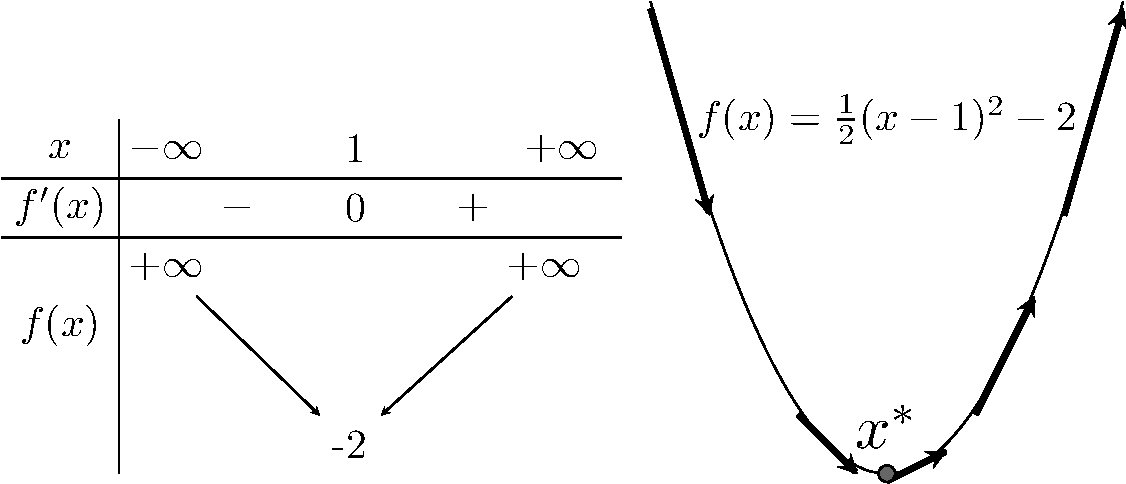
\includegraphics[width=.5\textwidth]{Chapters/04_Gradientdescent/GD/latex/gradient_descent.pdf}
    }
\end{figure}
% ******************************************************************************

% \index{local minimum}
% \index{global minimum}
\index{cực tiểu toàn cục -- global minima}
\index{cực đại toàn cục -- global maxima}
\index{cực trị toàn cục -- global extrema}

\index{cực tiểu địa phương -- local minima}
\index{cực đại địa phương -- local maxima}
\index{cực trị địa phương -- local extrema}
\def\mcd{\mathcal{D}}
\def\mcv{\mathcal{V}}
Xét một hàm số $f: \R^d \rightarrow \R$ với tập xác định $\mcd$,
\begin{itemize}
    \item Điểm $\bx^* \in \mcd$ được gọi là \textit{cực tiểu toàn cục} (tương ứng \textit{cực đại toàn cục}) nếu $f(\bx) \geq f(\bx^*)$ (tương ứng $f(\bx) \leq f(\bx^*)$) với mọi $\bx$ trong tập xác định $\mcd$. Các điểm cực tiểu toàn cục và cực đại toàn cục được gọi chung là \textit{cực trị toàn cục}.


    \item Điểm $\bx^* \in \mcd$ được gọi là \textit{cực tiểu địa phương} (tương ứng \textit{cực đại địa phương}) nếu tồn tại $\varepsilon > 0$ sao cho $f(\bx) \geq f(\bx^*)$ (tương ứng $f(\bx) \leq f(\bx^*)$) với mọi $\bx$ nằm trong lân cận $\mcv(\varepsilon) = \{\bx: \bx \in \mcd, d(\bx, \bx^*) \leq \varepsilon\}$. Ở đây $d(\bx, \bx^*)$ ký hiệu khoảng cách giữa hai vector $\bx$ và $\bx^*$, thường là khoảng cách Euclid. Các điểm cực tiểu địa phương và cực đại địa phương được gọi chung là \textit{cực trị địa phương}. Các điểm cực tiểu/cực đại/cực trị toàn cục cũng là các điểm cực tiểu/cực đại/cực trị địa phương. 
\end{itemize}



 
Giả sử ta đang quan tâm đến một hàm liên tục một biến có đạo hàm mọi nơi, xác
định trên $\R$. Cùng nhắc lại một vài điểm cơ bản:
\begin{itemize}
    \item Điểm cực tiểu địa phương $x^*$ của hàm số là điểm có đạo hàm $f'(x^*)$
    bằng không. Hơn nữa, trong lân cận của nó, đạo hàm của các điểm phía bên
    trái $x^*$ là không dương, đạo hàm của các điểm phía bên phải $x^*$ là không
    âm.

    \item Đường tiếp tuyến với đồ thị hàm số đó tại một điểm bất kỳ có hệ số góc
    bằng đạo hàm của hàm số tại điểm đó.
\end{itemize}
 
Hình \ref{fig:7_0} mô tả sự biến thiên của hàm số $f(x) = \frac{1}{2}(x - 1)^2 -
2$. Điểm $x^* = 1$ là một điểm cực tiểu toàn cục của hàm số này. Các điểm bên
trái của $\bx^*$ có đạo hàm âm, các điểm bên phải có đạo hàm dương. Với
hàm số này, càng xa về phía trái của $\bx^*$ thì đạo hàm càng âm, càng xa về
phía phải thì đạo hàm càng dương.
 
 
% \subsection{Gradient descent}
Trong machine learning nói riêng và toán tối ưu nói chung, chúng ta thường xuyên
phải tìm các cực tiểu toàn cục của một hàm số. Nếu chỉ xét riêng các hàm khả vi,
việc giải phương trình đạo hàm bằng không có thể phức tạp hoặc có vô số nghiệm.
Thay vào đó, người ta thường tìm các điểm cực tiểu địa phương, và coi đó là một
nghiệm cần tìm của bài toán trong những trường hợp nhất định.

Các điểm cực tiểu địa phương là nghiệm của phương trình đạo hàm bằng không (ta
vẫn đang giả sử rằng các hàm này liên tục và khả vi). Nếu tìm được toàn bộ (hữu
hạn) các điểm cực tiểu địa phương, ta chỉ cần thay từng điểm đó vào hàm số để
suy ra điểm cực tiểu toàn cục. Tuy nhiên, trong hầu hết các trường hợp, việc
giải phương trình đạo hàm bằng không là bất khả thi. Nguyên nhân có thể đến từ
sự phức tạp của đạo hàm, từ việc các điểm dữ liệu có số chiều lớn hoặc từ việc
có quá nhiều điểm dữ liệu. Thực tế cho thấy, trong nhiều bài toán machine
learning, các điểm cực tiểu địa phương thường cho kết quả tốt, đặc biệt là
trong các mạng neuron nhân tạo.

Một hướng tiếp cận phổ biến để giải quyết các bài toán tối ưu là dùng một phép
toán. Đầu tiên, chọn một \textit{điểm xuất phát} rồi tiến dần đến \textit{đích}
sau mỗi vòng lặp. Gradient descent (GD) và các biến thể của nó là một trong
những phương pháp được dùng nhiều nhất.

\textit{\textbf{Chú ý}}: Khái niệm \textit{nghiệm} của một bài toán tối ưu được sử dụng không hẳn để chỉ cực tiểu toàn cục. Nó được sử dụng theo nghĩa là kết quả của quá trình tối ưu. Kết quả ở một vòng lặp trung gian được gọi là \textit{vị trí của nghiệm}. Nói cách khác, \textit{nghiệm} có thể được hiểu là giá trị hiện tại của tham số cần tìm trong quá trình tối ưu. 
 
 
 
\section{Gradient descent cho hàm một biến}
Xét các hàm số một biến $f: \R \rightarrow \R$. Quay trở lại Hình~\ref{fig:7_0}
và một vài quan sát đã nêu. Giả sử  $x_{t}$ là điểm tìm được sau vòng lặp thứ
$t$. Ta cần tìm một thuật toán để đưa $x_{t}$ về càng gần $x^*$ càng tốt. Có hai
quan sát sau đây:
\begin{itemize}
    \item Nếu đạo hàm của hàm số tại $x_{t}$ là dương ($f'(x_{t}) > 0$) thì
    $x_t$ nằm
    về bên phải so với $x^*$, và ngược lại. Để điểm tiếp theo $x_{t+1}$ gần với
    $x^*$ hơn, ta cần di chuyển $x_t$ về bên trái, tức về phía
    \textit{âm}. Nói các khác, \textit{ta cần di chuyển $x_t$ ngược dấu với đạo hàm}:
    \begin{equation} 
    x_{t+1} = x_t + \Delta.
    \end{equation} 
    Trong đó $\Delta$ là một đại lượng ngược dấu với đạo hàm $f'(x_t)$. 
    
    \item $x_t$ càng xa $x^*$ về bên phải thì $f'(x_t)$ càng lớn (và
    ngược lại). Một cách tự nhiên nhất, ta chọn lượng di chuyển $\Delta$ tỉ lệ
    thuận với $-f'(x_t)$.
 \end{itemize} 
\index{tốc độ học -- learning rate}
Từ hai nhận xét trên, ta có công thức cập nhật đơn giản là
% \newnote{}{
% \boxed{
\begin{equation} 
\boxed{
x_{t+1} = x_t - \eta f'(x_t)
}
\end{equation} 
% }
% \boxed{a = 3}
% }
Trong đó $\eta$ là một số dương được gọi là \textit{tốc độ học}
(\textit{learning rate}). Dấu trừ thể hiện việc $x_t$ cần \textit{đi ngược} với
đạo hàm $f'(x_t)$. Tên gọi \textit{gradient descent} xuất phát từ đây\footnote{
\textit{Descent} nghĩa là \textit{đi ngược}}. Mặc dù các quan sát này không đúng
trong mọi trường hợp, chúng vẫn là nền tảng cho rất nhiều phương pháp tối ưu.
 
\subsection{Ví dụ đơn giản với Python}
 
Xét hàm số $f(x) = x^2 + 5\sin(x)$ với đạo hàm $f'(x) = 2x + 5\cos(x)$. Giả sử
xuất phát từ một điểm $x_{0}$, quy tắc cập nhật tại vòng lặp thứ $t$ là
\begin{equation} 
x_{t+1} = x_t - \eta(2x_t + 5\cos(x_t)). 
\end{equation} 
Khi thực hiện trên Python, ta cần viết các hàm số\footnote{Giả sử rằng các thư
viện đã được khai báo đầy đủ}:
\begin{enumerate}
    \item \pythoninline{grad} để tính đạo hàm. 

    \item  \pythoninline{cost} để tính giá trị của hàm số. Ta không sử dụng hàm này trong thuật toán cập nhật nghiệm. Tuy nhiên, nó vẫn đóng vai trò quan trọng trong việc kiểm tra tính chính xác của đạo hàm và sự biến thiên của hàm số sau mỗi vòng lặp.

    \item \pythoninline{myGD1} là phần chính thực hiện thuật toán GD. Đầu vào
    của hàm số này là điểm xuất phát \pythoninline{x0} và tốc độ học
    \pythoninline{eta}. Đầu ra là nghiệm của bài toán. Thuật toán dừng lại khi
    đạo hàm đủ nhỏ.
\end{enumerate}
 
 
\begin{lstlisting}[language=Python]
def grad(x): 
    return 2*x+ 5*np.cos(x) 
 
def cost(x): 
    return x**2 + 5*np.sin(x) 
\end{lstlisting}

\begin{lstlisting}[language=Python]
def myGD1(x0, eta): 
    x = [x0] 
    for it in range(100): 
        x_new = x[-1] - eta*grad(x[-1]) 
        if abs(grad(x_new)) < 1e-3: # just a small number 
            break 
        x.append(x_new) 
    return (x, it) 
\end{lstlisting}
 
 
 
\subsubsection{Điểm xuất phát khác nhau}
 
Sau khi đã có các hàm cần thiết, chúng ta thử tìm nghiệm với các điểm xuất phát
khác nhau là $x_{0} = -5$ và $x_{0} = 5$ với cùng tốc độ học $\eta = 0.1$.
 
\begin{lstlisting}[language=Python]
(x1, it1) = myGD1(-5, .1) 
(x2, it2) = myGD1(5, .1) 
print('Solution x1 = %f, cost = %f, after %d iterations'%(x1[-1], cost(x1[-1]), it1)) 
print('Solution x2 = %f, cost = %f, after %d iterations'%(x2[-1], cost(x2[-1]), it2)) 
\end{lstlisting}
\kq 
\begin{lstlisting}[language=Python]
Solution x1 = -1.110667, cost = -3.246394, after 11 iterations 
Solution x2 = -1.110341, cost = -3.246394, after 29 iterations 
\end{lstlisting} 
  
Như vậy, thuật toán trả về kết quả gần giống nhau với các điểm xuất phát khác
nhau, nhưng tốc độ hội tụ khác nhau. Hình~\ref{fig:7_1} và Hình~\ref{fig:7_2}
thể hiện vị trí của $x_t$ và đạo hàm qua các vòng lặp với cùng tốc độ học $\eta
= 0.1$ nhưng điểm xuất phát khác nhau tại $-5$ và $5$.
 

\begin{figure}[t]
\centering
    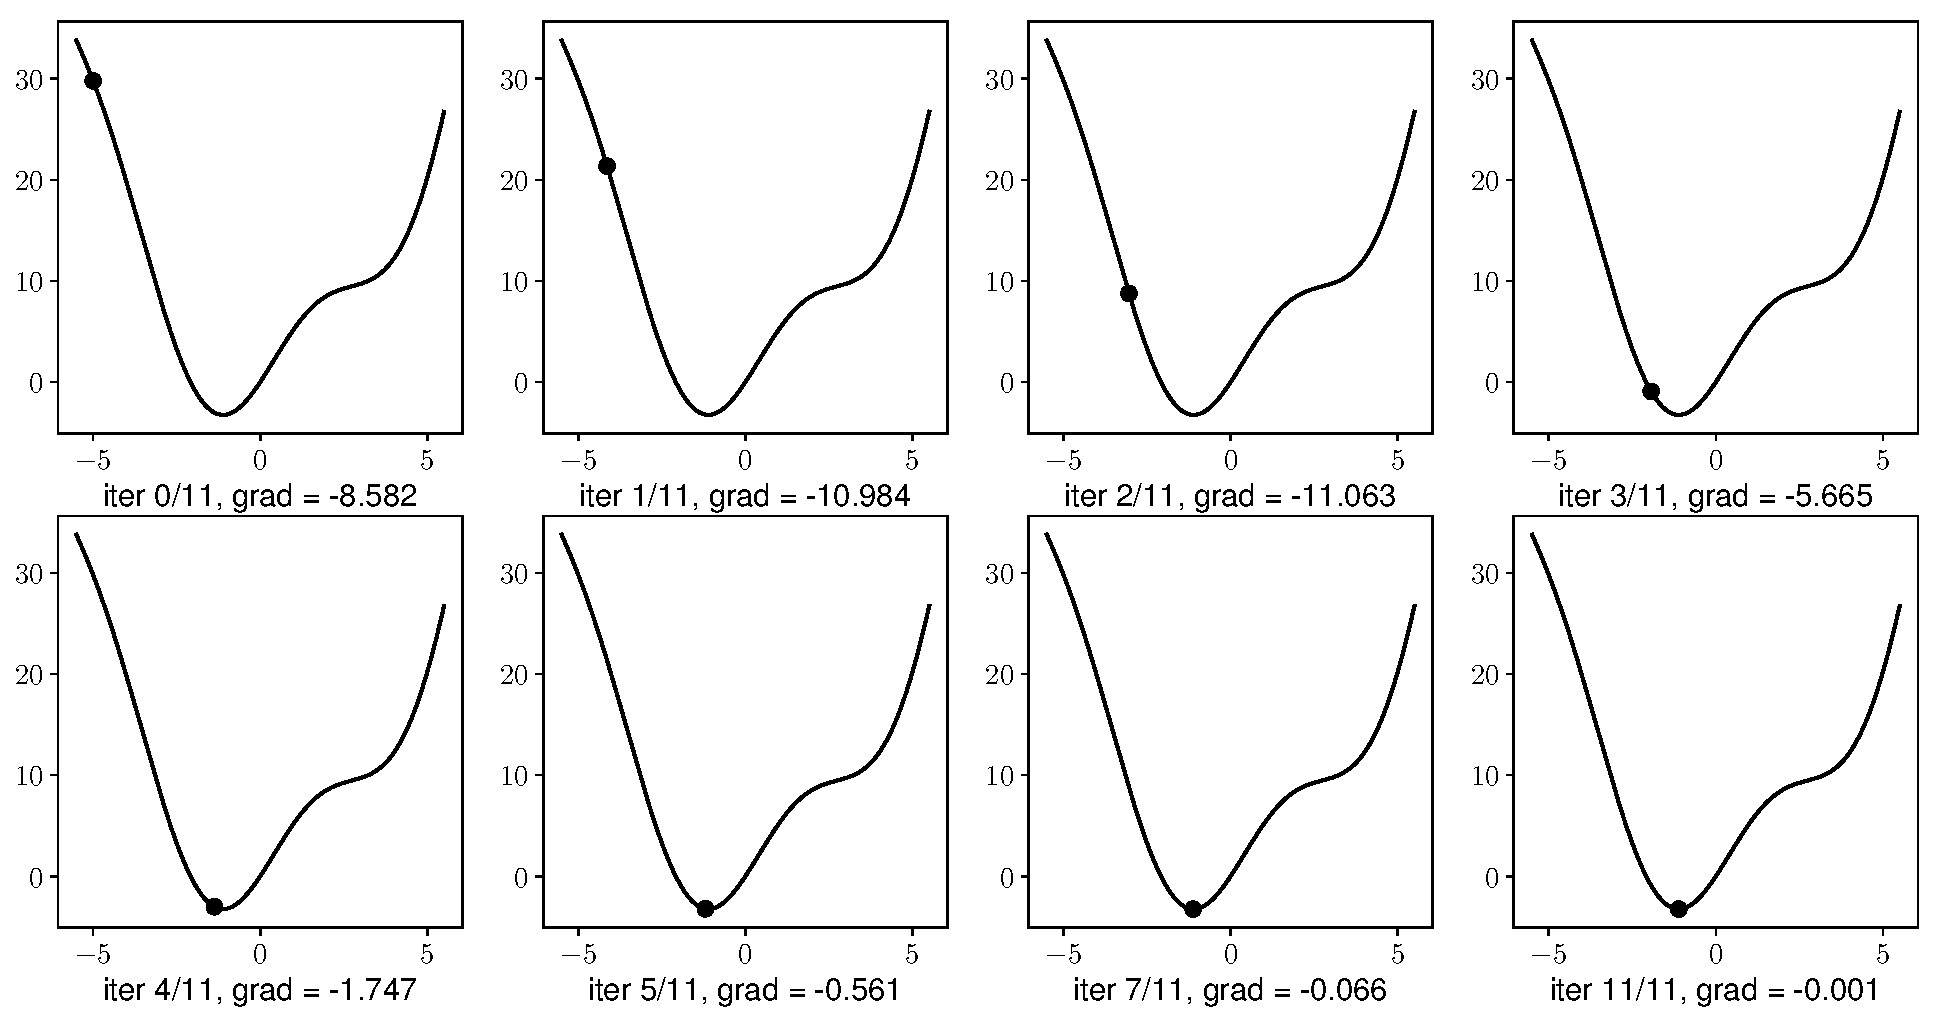
\includegraphics[width = \textwidth]{ebookML_src/src/grad_descent/gd1d_0.pdf}
    \caption[]{Kết quả tìm được qua các vòng lặp với $x_0 = -5, \eta = 0.1$}.
    \label{fig:7_1}
\end{figure}

\begin{figure}[t]
\centering
    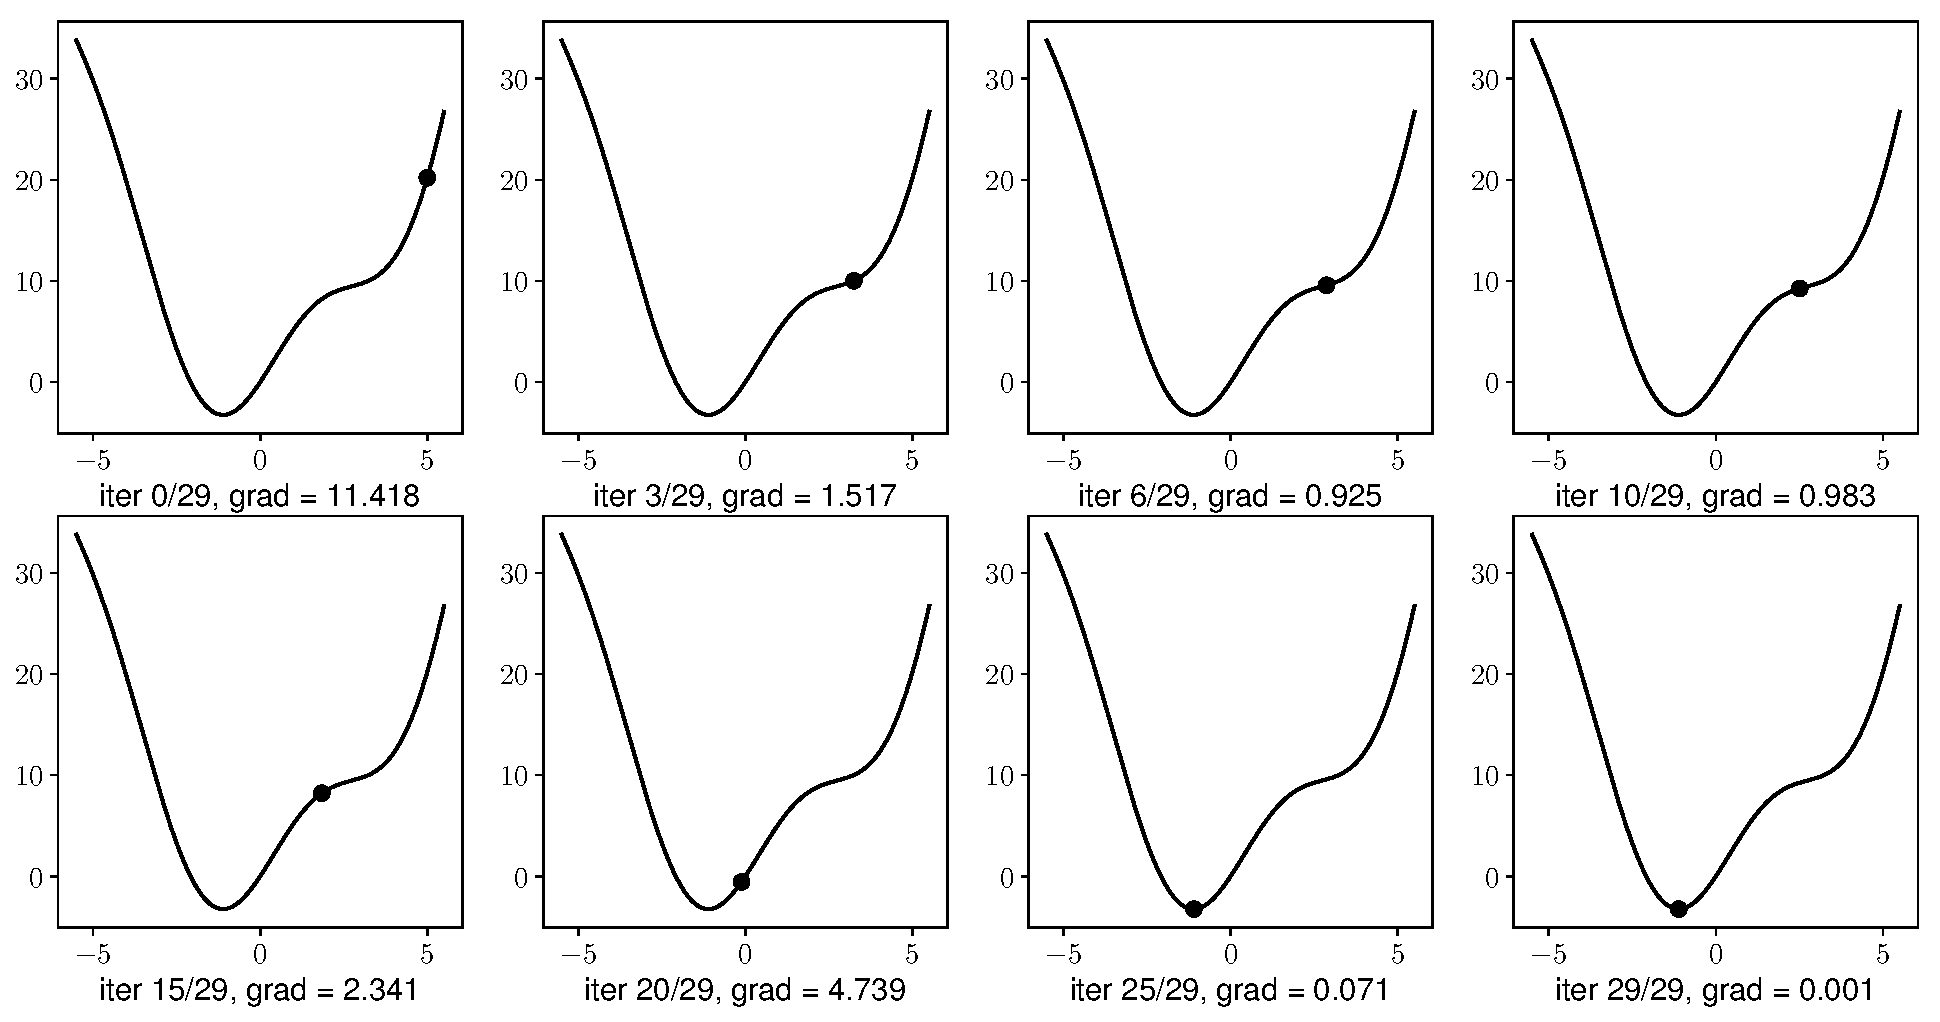
\includegraphics[width = \textwidth]{ebookML_src/src/grad_descent/gd1d_3.pdf}
    \caption[]{Kết quả tìm được qua các vòng lặp với $x_0 = 5, \eta = 0.1$}.
    \label{fig:7_2}
\end{figure}


% \begin{figure}[t]
% \centering
%     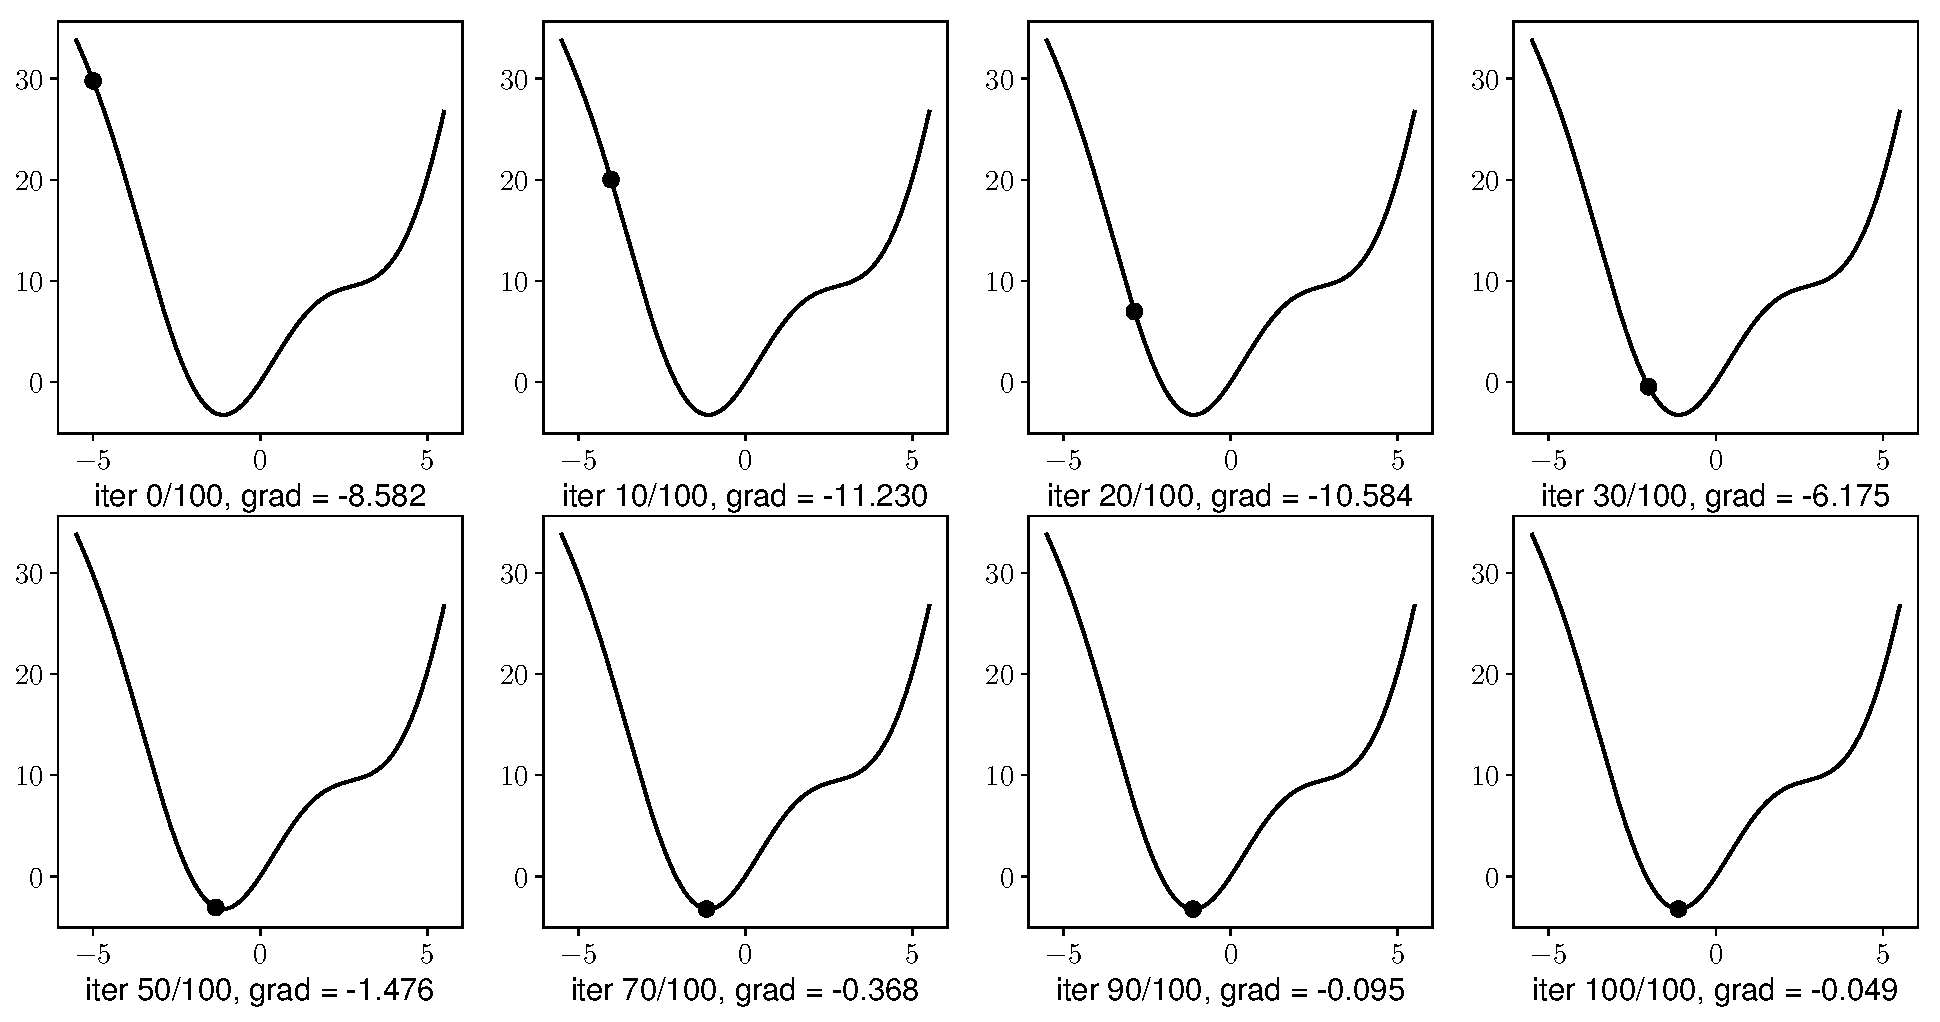
\includegraphics[width = \textwidth]{ebookML_src/src/grad_descent/gd1d_1.pdf}
%     \caption[]{s}
%     \label{fig:7_1}
% \end{figure}

% \begin{figure}[t]
% \centering
%     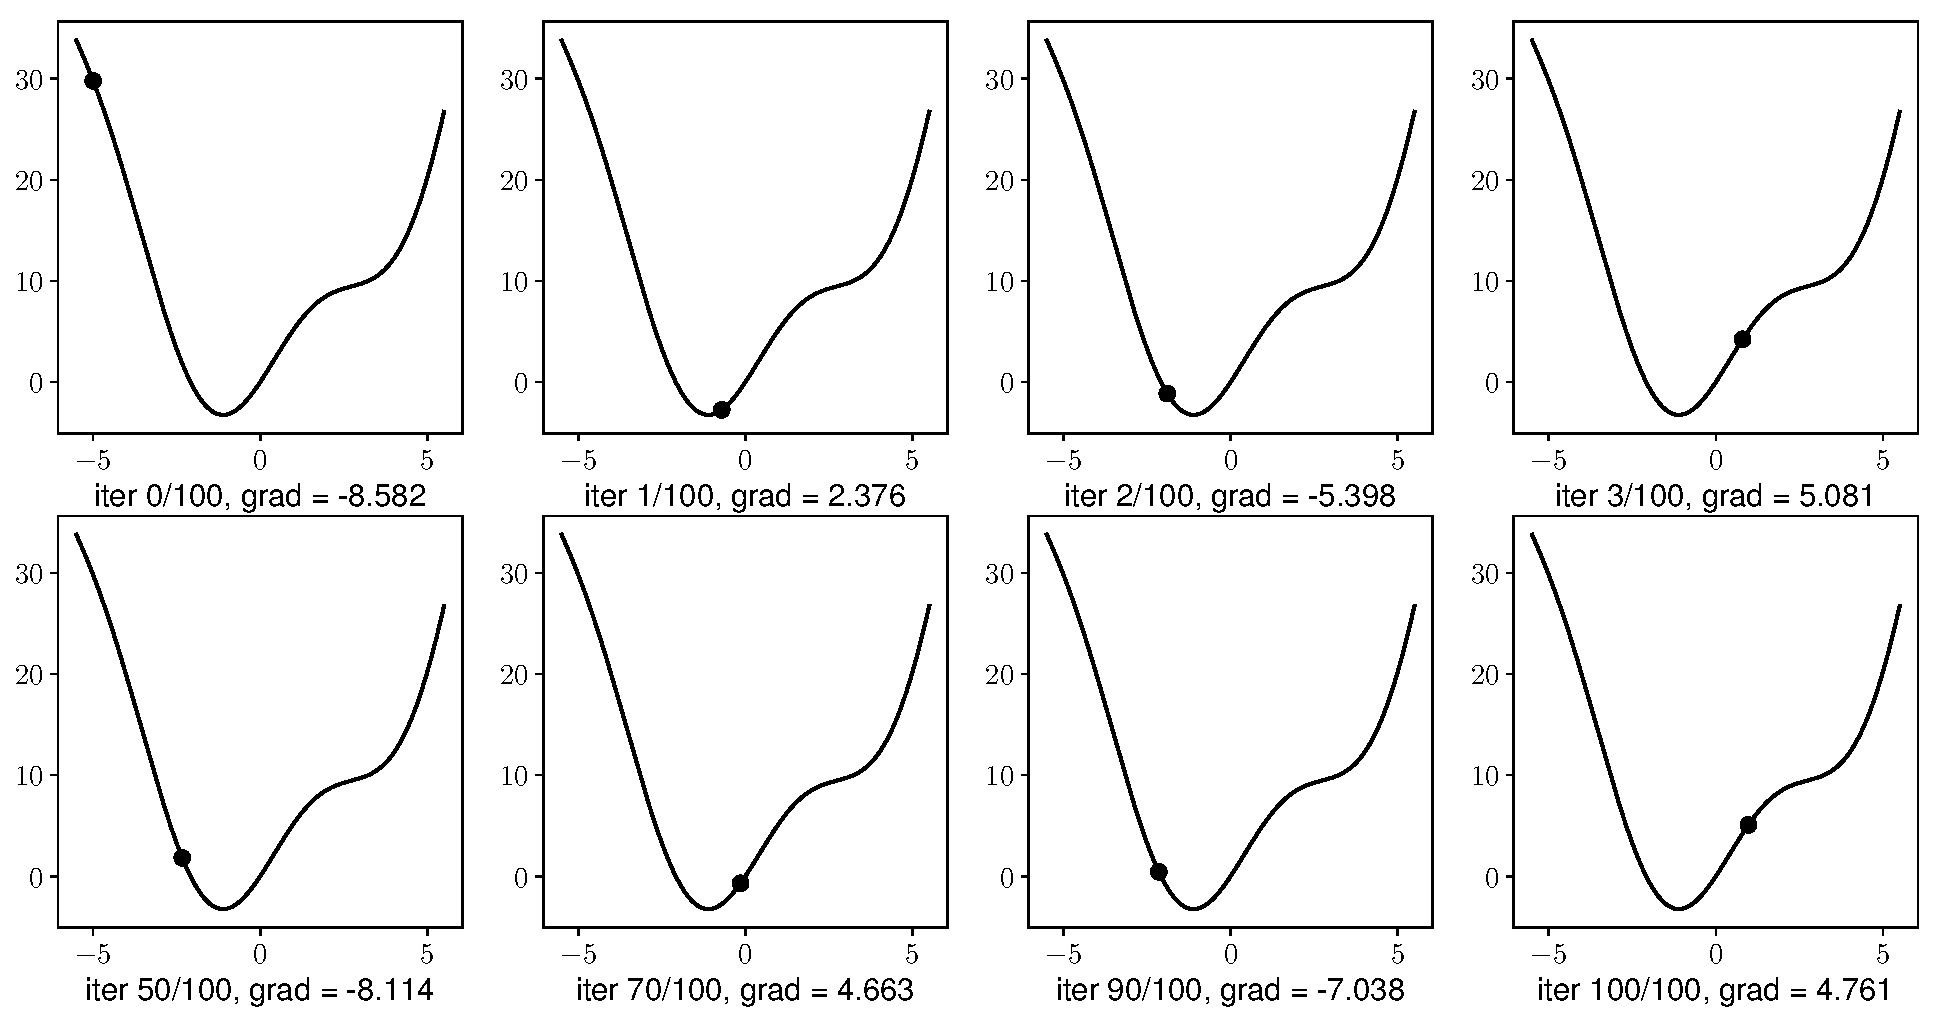
\includegraphics[width = \textwidth]{ebookML_src/src/grad_descent/gd1d_2.pdf}
%     \caption[]{s}
%     \label{fig:7_1}
% \end{figure}

% \begin{figure}[t]
% \centering
%     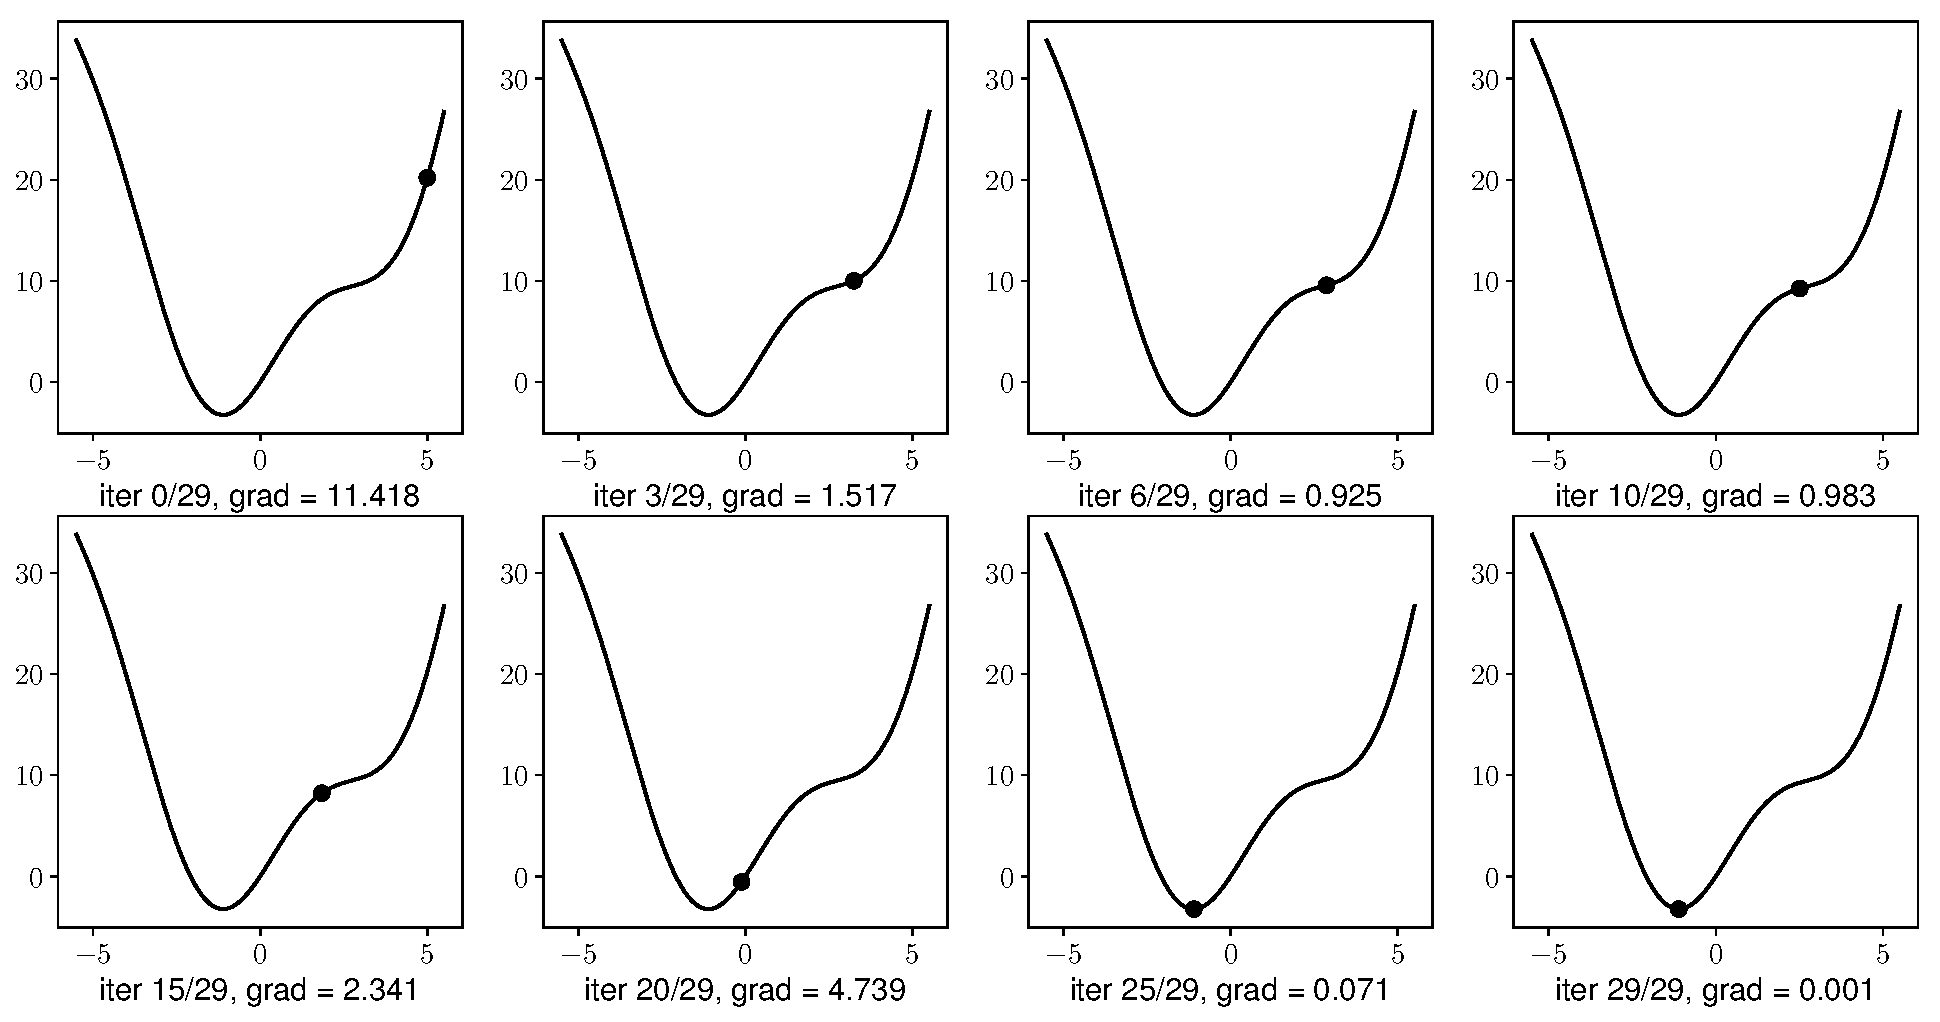
\includegraphics[width = \textwidth]{ebookML_src/src/grad_descent/gd1d_3.pdf}
%     \caption[]{s}
%     \label{fig:7_1}
% \end{figure}
 
% <table width = "100%" style = "border: 0px solid white"> 
%    <tr > 
%         <td width="50%" style = "border: 0px solid white">  
%             <img style="display:block;" width = "100%" src = "/assets/GD/1dimg_5_0.1_-5.gif"> 
%         </td> 
%         <td width="50%" style = "border: 0px solid white"> 
%             <img style="display:block;" width = "100%" src = "/assets/GD/1dimg_5_0.1_5.gif"> 
%         </td> 
%     </tr> 
% </table>  
% {\color{red} Hình động}
 
Hình~\ref{fig:7_1} tương ứng với $x_{0} = -5$, thuật toán hội tụ nhanh hơn. Hơn
nữa, {đường đi} tới đích khá suôn sẻ với đạo hàm luôn âm và trị tuyệt đối của
đạo hàm nhỏ dần khi $x_t$ tiến gần tới đích.

Hình~\ref{fig:7_2} tương ứng với $x_{0} = 5 $, {đường đi} của $x_t$ chứa một
khu vực có đạo hàm khá nhỏ gần điểm có hoành độ bằng 2.5. Điều này khiến thuật
toán {la cà} ở đây khá lâu. Khi vượt qua được điểm này thì mọi việc diễn ra tốt
đẹp. Các điểm không phải là điểm cực tiểu nhưng có đạo hàm gần bằng không rất dễ
gây ra hiện tượng $x_t$ bị \textit{bẫy} vì đạo hàm nhỏ khiến nó không thay đổi
nhiều ở vòng lặp tiếp theo. Chúng ta sẽ thấy một kỹ thuật khác giúp thuật toán
\textit{thoát} những chiếc bẫy này.
 
\subsubsection{Tốc độ học khác nhau}


\begin{figure}[t]
\centering
    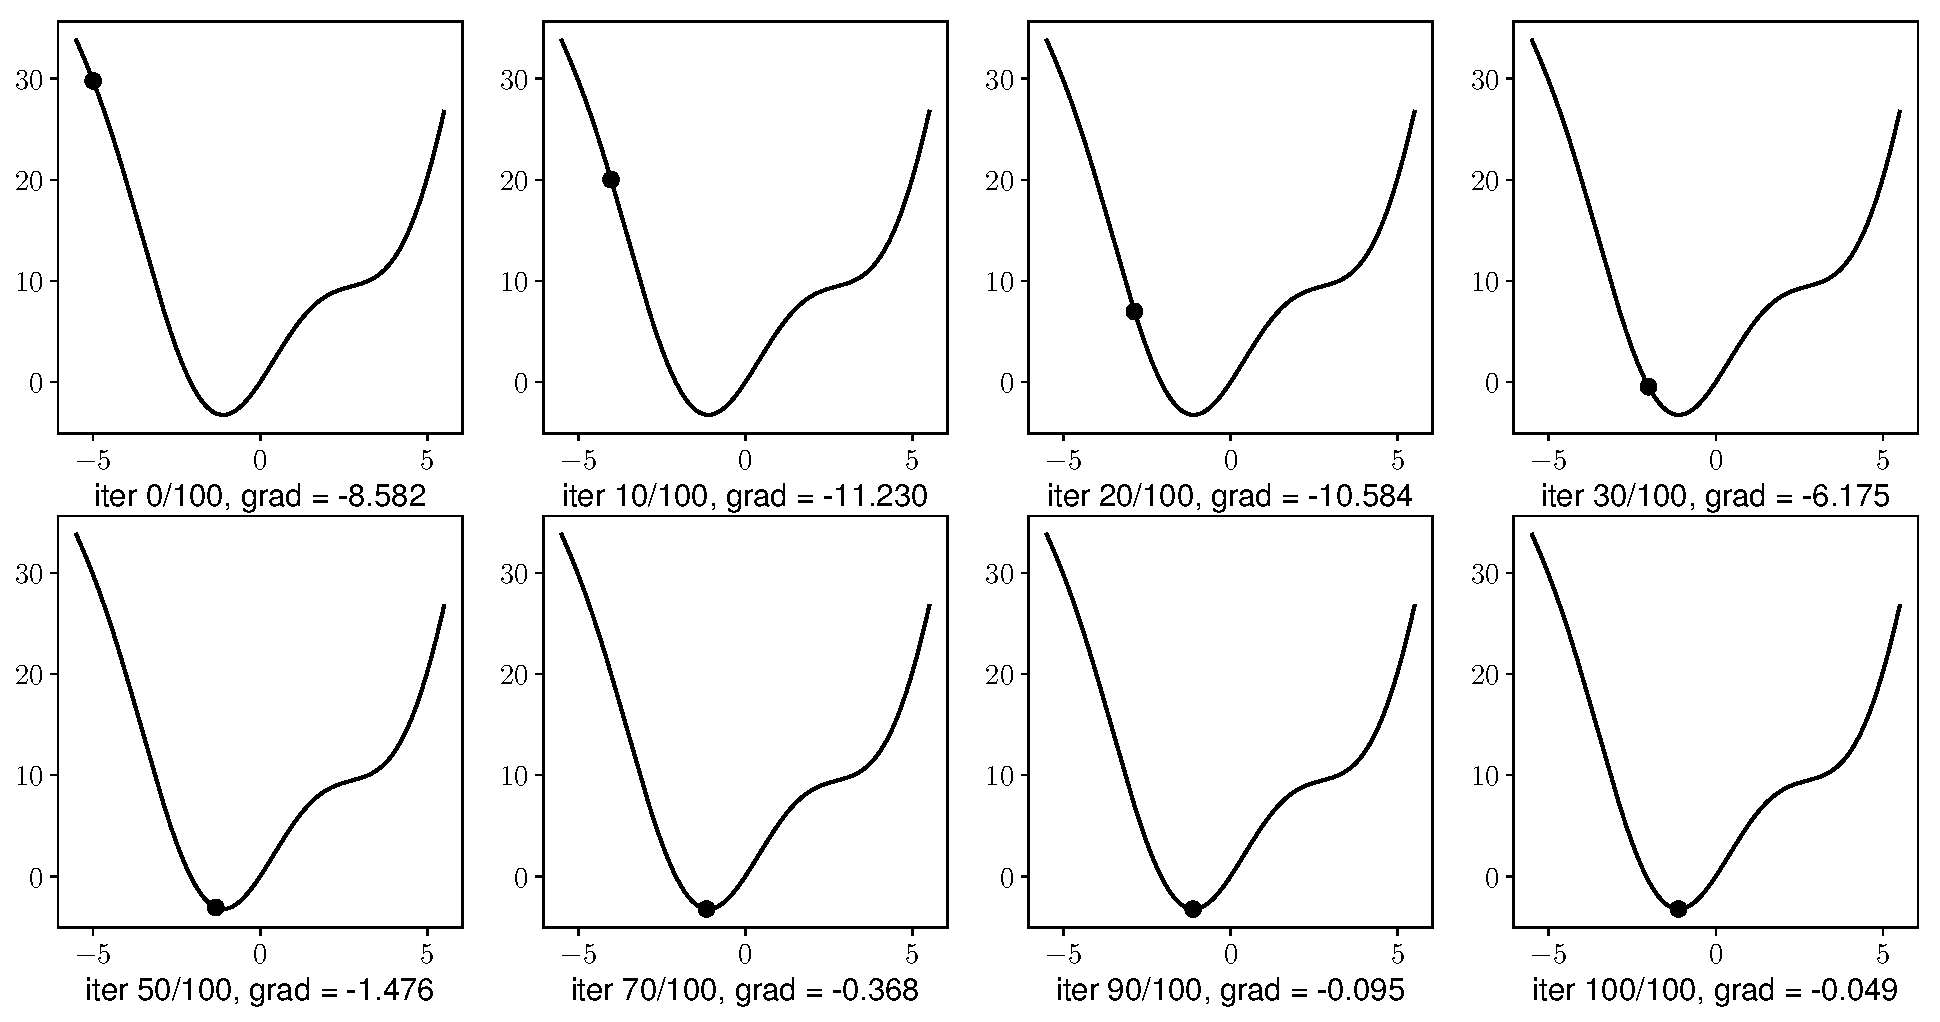
\includegraphics[width =
    .975\textwidth]{ebookML_src/src/grad_descent/gd1d_1.pdf}
    \caption[]{Kết quả tìm được qua các vòng lặp với $x_0 = -5$, $\eta = 0.01$.}
    \label{fig:7_3}
\end{figure}

\begin{figure}[t]
\centering
    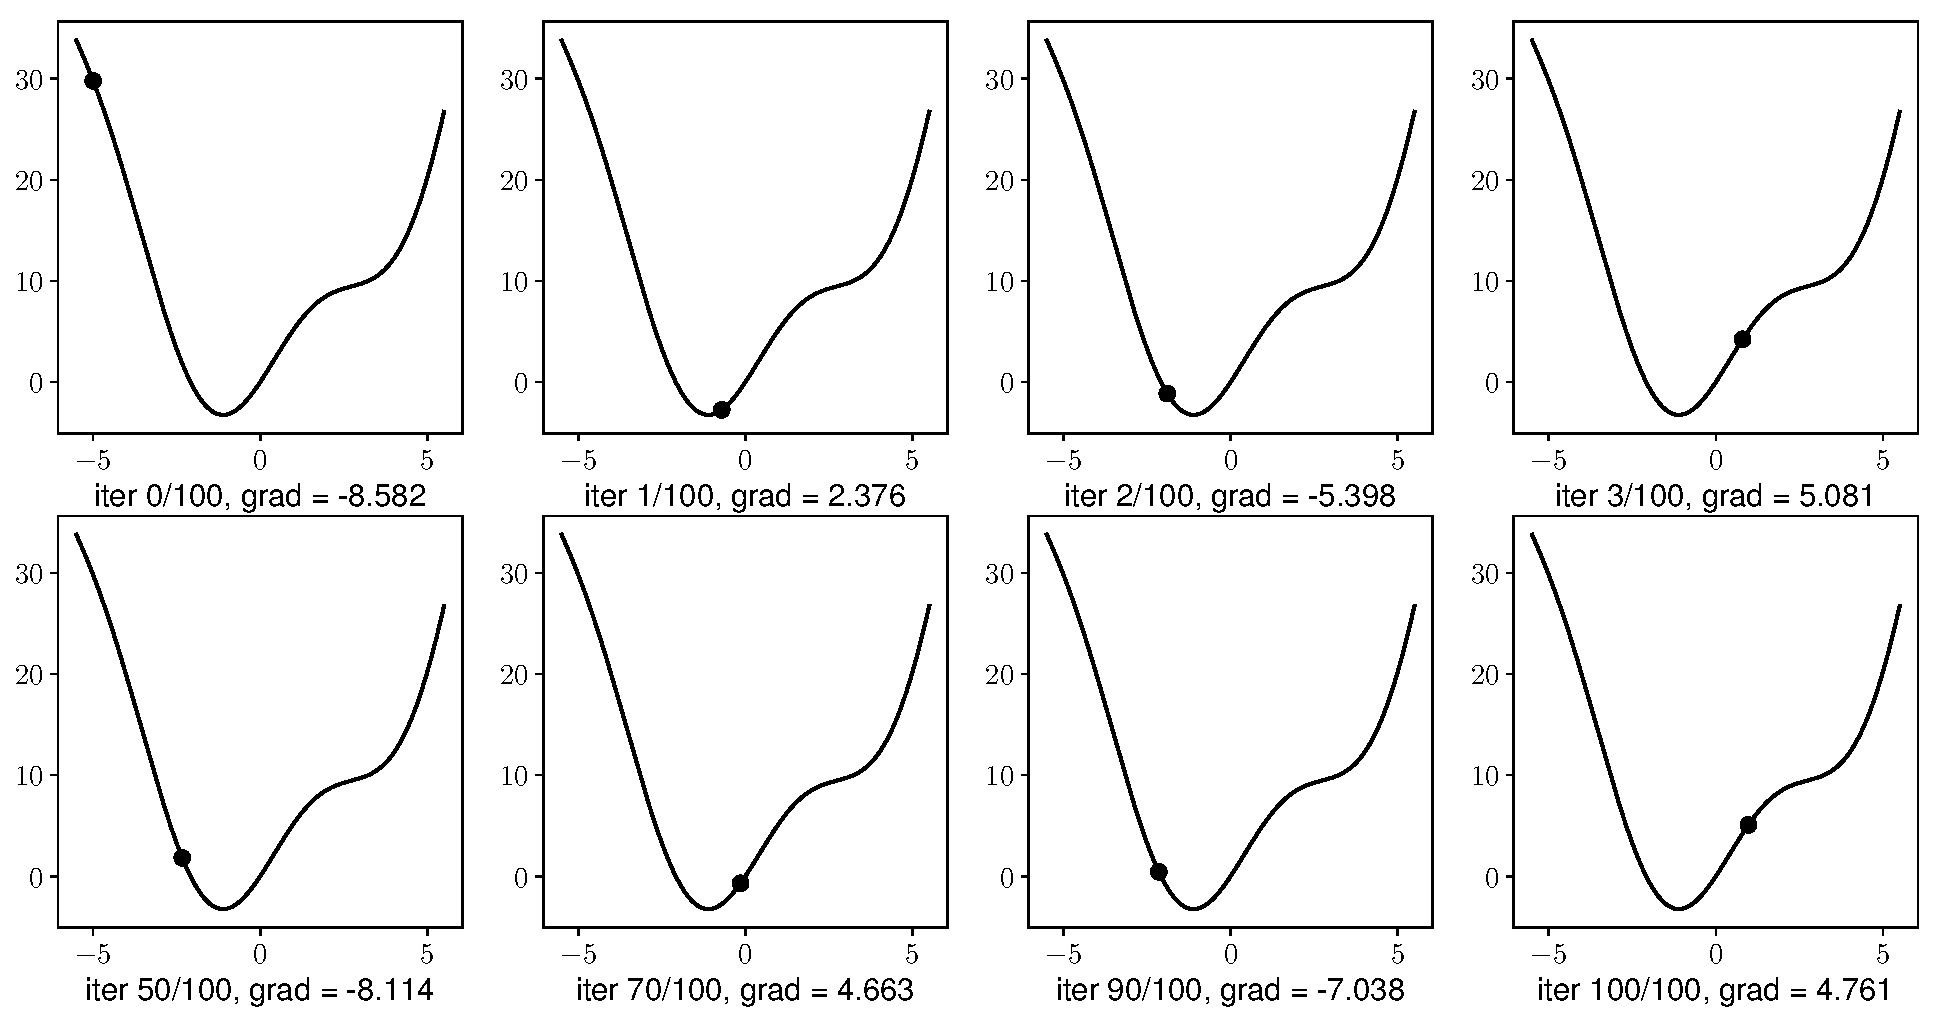
\includegraphics[width =
    .975\textwidth]{ebookML_src/src/grad_descent/gd1d_2.pdf}
    \caption[]{Kết quả tìm được qua các vòng lặp với $x_0 = -5, \eta = 0.5$}.
    \label{fig:7_4}
\end{figure}



Tốc độ hội tụ của GD không những phụ thuộc vào điểm xuất phát mà còn phụ
thuộc vào tốc độ học. Hình~\ref{fig:7_3} và Hình~\ref{fig:7_4} thể
hiện vị trí của $x_t$ qua các vòng lặp với cùng điểm xuất phát $x_{0} = -5$
nhưng tốc độ học khác nhau. Ta quan sát thấy hai điều: 
\begin{itemize}
    \item Với tốc độ học nhỏ $\eta = 0.01$ (Hình~\ref{fig:7_3}), tốc độ
    hội tụ rất chậm. Trong ví dụ này ta chọn tối đa 100 vòng lặp nên thuật toán
    dừng lại trước khi tới {đích}, mặc dù đã rất gần. Trong thực tế, khi việc
    tính toán trở nên phức tạp, tốc độ học quá thấp sẽ ảnh hưởng nhiều tới tốc
    độ của thuật toán. Thậm chí $x_t$ có thể không bao giờ tới được đích.

    \item Với tốc độ học lớn $\eta = 0.5$ (Hình~\ref{fig:7_4}),
    $x_t$ tiến nhanh tới {gần đích} sau vài vòng lặp. Tuy nhiên,
    thuật toán không hội tụ được vì sự thay đổi vị trí của $x_t$ sau mỗi vòng
    lặp là quá lớn, khiến $x_t$ dao động quanh đích nhưng không tới được đích. 

\end{itemize}
\index{suy giảm tốc độ học -- learning rate decay}
Việc lựa chọn tốc độ học rất quan trọng. Tốc độ học thường được chọn thông qua
các thí nghiệm. Ngoài ra, GD có thể làm việc hiệu quả hơn bằng cách chọn tốc độ
học khác nhau ở mỗi vòng lặp. Trên thực tế, một kỹ thuật thường được sử dụng có
tên là \textit{suy giảm tốc độ học} (\textit{learning rate decay}). Trong kỹ
thuật này, tốc độ học được giảm đi sau một vài vòng lặp để nghiệm không bị dao
động mạnh khi gần đích hơn.
 
 
\section{Gradient descent cho hàm nhiều biến}
Giả sử ta cần tìm cực tiểu toàn cục cho hàm $f(\mathbf{\theta})$ trong đó
$\mathbf{\theta}$ là tập hợp các tham số cần tối ưu. Gradient\footnote{Với các
biến nhiều chiều, chúng ta sẽ sử dụng \textit{gradient} thay cho \textit{đạo
hàm}.} của hàm số đó tại một điểm $\theta$ bất kỳ được ký hiệu là
$\nabla_{\theta}f(\theta)$. Tương tự như hàm một biến, thuật toán GD cho hàm
nhiều biến cũng bắt đầu bằng một điểm dự đoán $\theta_{0}$, sau đó sử dụng quy
tắc cập nhật
\begin{equation} 
\boxed{
\theta_{t+1} = \theta_{t} - \eta \nabla_{\theta} f(\theta_{t}) 
}
\end{equation} 
Hoặc viết dưới dạng đơn giản hơn: $\theta \assign \theta - \eta \nabla_{\theta}
f(\theta)$.
 
% Quy tắc cần nhớ: \textbf{luôn luôn đi ngược hướng với đạo hàm}. 
 
% Việc tính toán đạo hàm của các hàm nhiều biến là một kỹ năng cần thiết. Một vài đạo hàm đơn giản có thể được \href{http://machinelearningcoban.com/math/#bang-cac-dao-ham-co-ban}{tìm thấy ở đây}. 
 
\subsubsection{Quay lại với bài toán hồi quy tuyến tính}

Trong mục này, chúng ta quay lại với bài toán hồi quy tuyến tính và thử tối ưu
hàm mất mát của nó bằng thuật toán GD.
 
Nhắc lại hàm mất mát của hồi quy tuyến tính và gradient theo $\bw$:
\begin{equation} 
\mathcal{L}(\mathbf{w}) = \frac{1}{2N}\|\by - \bX^T\bw\|_2^2; \quad \nabla_{\mathbf{w}}\mathcal{L}(\mathbf{w}) =  
\frac{1}{N}\bX(\bX^T\bw - \by) 
\end{equation} 

  
\subsubsection{Ví dụ trên Python và một vài lưu ý khi lập trình}
 
% Load thư viện 
 
 
% \begin{lstlisting}[language=Python]
% # To support both python 2 and python 3 
% from __future__ import division, print_function, unicode_literals 
% import numpy as np  
% import matplotlib 
% import matplotlib.pyplot as plt 
% np.random.seed(2) 
% \end{lstlisting}
 
Trước tiên, chúng ta tạo 1000 điểm dữ liệu gần đường thẳng $y = 4 + 3x$ rồi dùng thư viện scikit-learn để tìm nghiệm cho hồi quy tuyến tính:
  
\begin{lstlisting}[language=Python]
from sklearn.linear_model import LinearRegression 
X = np.random.rand(1000)
y = 4 + 3 * X + .5*np.random.randn(1000) # noise added
model = LinearRegression()
model.fit(X.reshape(-1, 1), y.reshape(-1, 1))
w, b = model.coef_[0][0], model.intercept_[0]
sol_sklearn = np.array([b, w])
print(sol_sklearn)
\end{lstlisting}
Kết quả:
\begin{lstlisting}
Solution found by sklearn: [ 3.94323245  3.12067542]
\end{lstlisting}
 
 
% <div class="imgcap"> 
%  <img src ="/assets/GD/output_11_1.png" align = "center" width = "400"> 
% </div> 
\begin{figure}[t]
     % caption on side     
     \floatbox[{\capbeside\thisfloatsetup{capbesideposition={right,top},capbesidewidth=6cm}}]{figure}[\FBwidth]
     {\caption{ 
     Nghiệm của bài toán hồi quy tuyến tính (đường thằng màu đen) tìm được bằng
     thư viện scikit-learn.
     }
     \label{fig:7_lr_sklearn}}
     { % figure here
    
     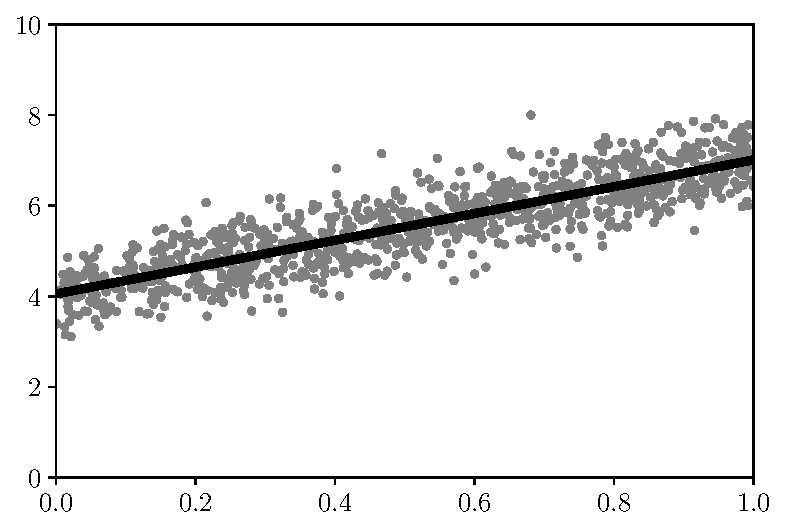
\includegraphics[width=.485\textwidth]{ebookML_src/src/grad_descent/LR_data.pdf}
     }
 \end{figure}
Các điểm dữ liệu và đường thẳng tìm được bằng hồi quy tuyến tính có phương trình
$y \approx 3.94 + 3.12x$ được minh hoạ trong Hình~\ref{fig:7_lr_sklearn}. Nghiệm
tìm này được rất gần với mong đợi.
 
Tiếp theo, ta sẽ thực hiện tìm nghiệm bằng GD. Ta cần viết hàm mất mát và gradient theo $\bw$. Chú ý rằng ở đây $\bw$ đã bao gồm hệ số điều chỉnh $b$.
 
\begin{lstlisting}[language=Python]
def grad(w):
    N = Xbar.shape[0]
    return 1/N * Xbar.T.dot(Xbar.dot(w) - y)

def cost(w):
    N = Xbar.shape[0]
    return .5/N*np.linalg.norm(y - Xbar.dot(w))**2
\end{lstlisting}

Với các hàm phức tạp, chúng ta cần kiểm tra độ chính xác của gradient thông
qua numerical gradient (xem Mục~\ref{sec:check_grad}). Phần kiểm tra này xin giành lại cho bạn đọc. Dưới đây là thuật toán GD cho bài toán.
 
\begin{lstlisting}[language=Python]
def myGD(w_init, grad, eta):
    w = [w_init]
    for it in range(100):
        w_new = w[-1] - eta*grad(w[-1])
        if np.linalg.norm(grad(w_new))/len(w_new) < 1e-3:
            break 
        w.append(w_new)
    return (w, it)

one = np.ones((X.shape[0],1))
Xbar = np.concatenate((one, X.reshape(-1, 1)), axis = 1)
w_init = np.array([[2], [1]])
(w1, it1) = myGD(w_init, grad, 1)
print('Sol found by GD: w = ', w1[-1].T, ', after %d iterations.' %(it1+1))
\end{lstlisting}
\kq 
\begin{lstlisting}[language=Python]
Sol found by GD: w =  [ 3.99026984  2.98702942] , after 49 iterations.
\end{lstlisting}
 
Thuật toán hội tụ tới kết quả khá gần với nghiệm tìm được theo scikit-learn sau
49 vòng lặp. Hình~\ref{fig:7_lrgd} mô tả đường đi của $\bw$ với cùng điểm xuất
phát nhưng tốc độ học khác nhau. Các điểm được đánh dấu `start' là các điểm xuất
phát. Các điểm được đánh dấu `destination' là nghiệm tìm được bằng thư viện
scikit-learn. Các điểm hình tròn nhỏ màu đen là vị trí của $\bw$ qua các vòng
lặp trung gian. Ta thấy rằng khi $\eta = 1$, thuật toán hội tụ tới rất gần đích
theo thư viện sau 49 vòng lặp. Với tốc độ học nhỏ hơn, $\eta = 0.1$, nghiệm vẫn
còn cách xa đích sau hơn 100 vòng lặp. Như vậy, việc chọn tốc độ học hợp lý là
rất quan trọng.


\begin{figure}[t]
    \begin{subfigure}{0.495\textwidth}
    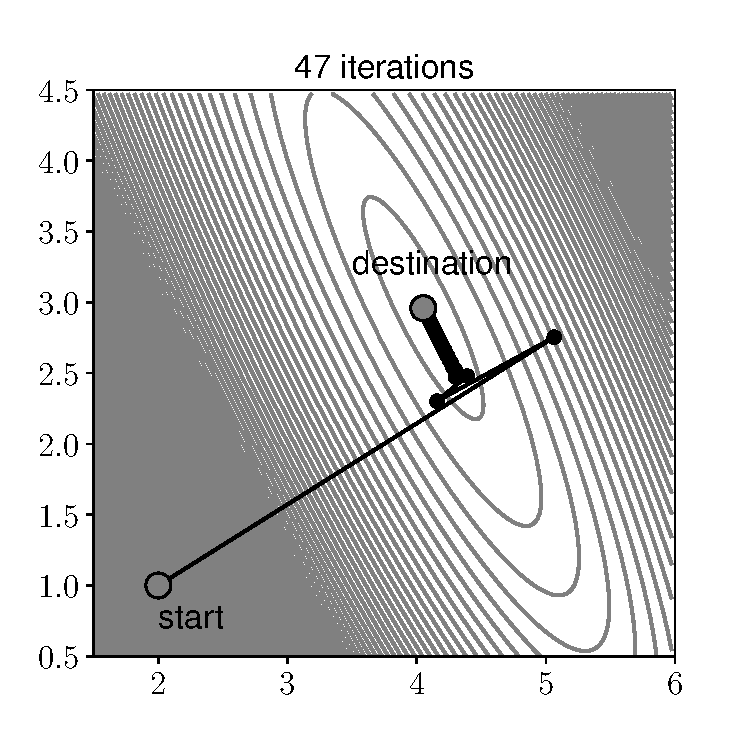
\includegraphics[width=0.99\linewidth]{ebookML_src/src/grad_descent/LR_gd_1.pdf}
    \caption{$\eta = 1$.}
    \label{fig:7_lrgda}
    \end{subfigure}
    \begin{subfigure}{0.495\textwidth}
    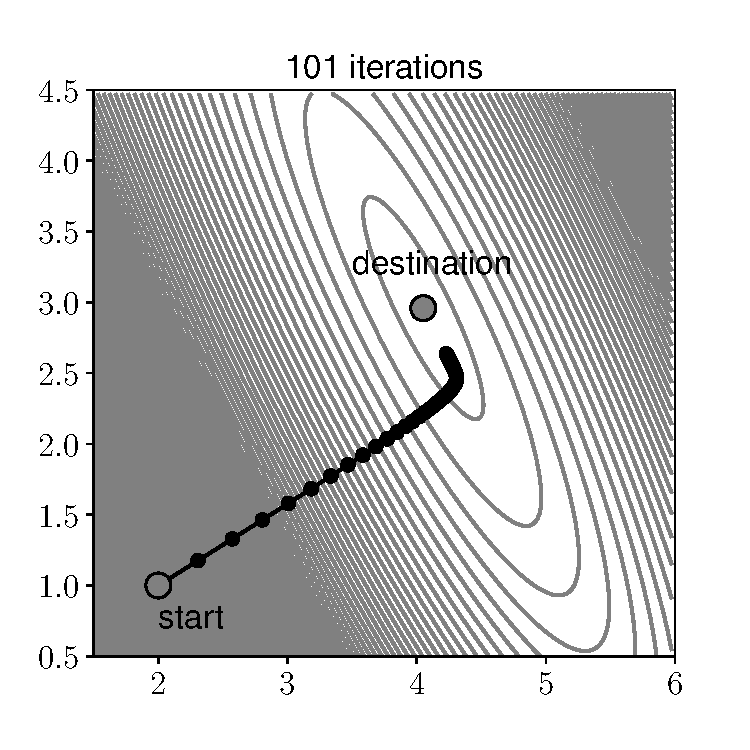
\includegraphics[width=0.99\linewidth]{ebookML_src/src/grad_descent/LR_gd_2.pdf}
    \caption{$\eta = 0.1$.}
    \label{fig:7_lrgdb}
    \end{subfigure}
    \caption{
    Đường đi nghiệm của hồi quy tuyến tính với các tốc độ học khác nhau. 
    }
    \label{fig:7_lrgd}
\end{figure}

\index{duo@đường đồng mức -- level sets}
Ở đây, chúng ta cùng làm quen với một khái niệm quan trọng: \textit{đường đồng
mức}. Khái niệm này thường xuất hiện trong các bản đồ tự nhiên. Với các ngọn
núi, đường đồng mức là các đường kín bao quanh đỉnh núi, bao gồm các điểm có
cùng độ cao so với mực nước biển. Khái niệm tương tự cũng được sử dụng trong tối
ưu. {Đường đồng mức} của một hàm số là tập hợp các điểm làm cho hàm số có cùng
giá trị. Xét một hàm số hai biến với đồ thị là một {bề mặt} trong
không gian ba chiều. Các đường đồng mức là giao điểm của bề mặt này với các mặt
phẳng song song với đáy. Hàm mất mát của hồi quy tuyến tính với dữ liệu một
chiều là một hàm bậc hai theo hai thành phần trong vector trọng số $\bw$. Đồ thị
của nó là một bề mặt parabolic. Vì vậy, các đường đồng mức của hàm này là các
đường ellipse có cùng tâm như trên Hình~\ref{fig:7_lrgd}. Tâm này chính là đáy
của parabolic và là giá trị nhỏ nhất của hàm mất mát. Các đường đồng mức càng
gần {tâm} ('destination') tương ứng với giá trị càng thấp.% đỏ đậm thể hiện giá trị tăng dần.% Nếu các bạn để ý trong các bản độ tự nhiên, để miêu tả độ cao của các dãy núi, người ta dùng nhiều đường cong kín bao quanh nhau như sau: 
 
% <div class="imgcap"> 
%  <img src ="http://files.vforum.vn/2016/T06/img/vforum.vn-324944-hinh-44-lc6b0e1bba3c-c491e1bb93-c491e1bb8ba-hc3acnh-te1bb89-le1bb87-le1bb9bn.png" align = "center" width = "600"> 
%  <div class = "thecap"> Ví dụ về đường đồng mức trong các bản đồ tự nhiên. (Nguồn: <a href = "http://vforum.vn/diendan/showthread.php?90166-Dia-ly-6-Duong-dong-muc-la-nhung-duong-nhu-the-nao-">Địa lý 6: Đường đồng mức là những đường như thế nào?</a>)</div> 
% </div> 
 
 
% Các vòng nhỏ màu đỏ hơn thể hiện các điểm ở trên cao hơn.  
 
% Trong toán tối ưu, người ta cũng dùng phương pháp này để thể hiện các bề mặt trong không gian hai chiều.  
 
% Quay trở lại với hình minh họa thuật toán GD cho bài toán Liner Regression bên trên, hình bên phải là hình biểu diễn các level sets. Tức là tại các điểm trên cùng một vòng, hàm mất mát có giá trị như nhau. Trong ví dụ này, tôi hiển thị giá trị của hàm số tại một số vòng. Các vòng màu xanh có giá trị thấp, các vòng tròn màu đỏ phía ngoài có giá trị cao hơn. Điểm này khác một chút so với đường đồng mức trong tự nhiên là các vòng bên trong thường thể hiện một thung lũng hơn là một đỉnh núi (vì chúng ta đang đi tìm giá trị nhỏ nhất). 
 
% Thử với tốc độ học nhỏ hơn, kết quả như sau: 
 
% <table width = "100%" style = "border: 0px solid white"> 
%    <tr > 
%         <td width="40%" style = "border: 0px solid white">  
%         <img style="display:block;" width = "100%" src = "/assets/GD/img1_0.1.gif"> 
%          </td> 
%         <td width="40%" style = "border: 0px solid white"> 
%         <img style="display:block;" width = "100%" src = "/assets/GD/img2_0.1.gif"> 
%         </td> 
%     </tr> 
% </table>  
% {\color{red} HÌnh 7.6} 


% Tốc độ hội tụ đã chậm đi nhiều, thậm chí sau 99 vòng lặp, GD vẫn chưa tới gần được nghiệm tốt nhất. Trong các bài toán thực tế, chúng ta cần nhiều vòng lặp hơn 99 rất nhiều, vì số chiều và số điểm dữ liệu thường là rất lớn. 


% \section{Các thuật toán cải thiện Gradient descent}
\newpage
\section{Gradient descent với momentum}
\index{gradient descent!momentum}
 
% \subsection{Momentum}
 
% \subsubsection{Nhắc lại thuật toán Gradient descent}
% Dành cho các bạn chưa đọc \href{http://machinelearningcoban.com/2017/01/12/gradientdescent/}{phần 1} của Gradient descent. Để giải bài toán tìm điểm \textit{global optimal} của hàm mất mát $J(\theta)$ (Hàm mất mát cũng thường được ký hiệu là $J()$ với $\theta$ là tập hợp các tham số của mô hình), tôi xin nhắc lại thuật toán GD: 
 
Trước hết, nhắc lại thuật toán GD để tối ưu một hàm mất mát $J(\theta)$:
\begin{itemize}
    \item  Dự đoán một điểm xuất phát $\theta = \theta_0$. 
    \item  Cập nhật $\theta$ theo công thức
\begin{equation} 
\theta \assign \theta - \eta \nabla_{\theta}J(\theta) 
\end{equation}
tới khi hội tụ. Ở đây, $\nabla_{\theta}J(\theta)$ là gradient của hàm mất mát tại $\theta$. 
\end{itemize}
 
 
\subsubsection{Gradient dưới góc nhìn vật lý }
 
Thuật toán GD thường được ví với tác dụng của trọng lực lên một hòn bi đặt trên
một mặt có dạng thung lũng như Hình \ref{fig:8_1}a. Bất kể ta đặt hòn bi ở A
hay B thì cuối cùng nó cũng sẽ lăn xuống và kết thúc ở vị trí C.
 
% <div class="imgcap"> 
%  <img src ="/assets/GD/momentum.png" align = "center" width = "800"> 
%  <div class = "thecap"> Hình 1: So sánh Gradient descent với các hiện tượng vật lý </div> 
% </div> 
\begin{figure}[t]
\centering
    % 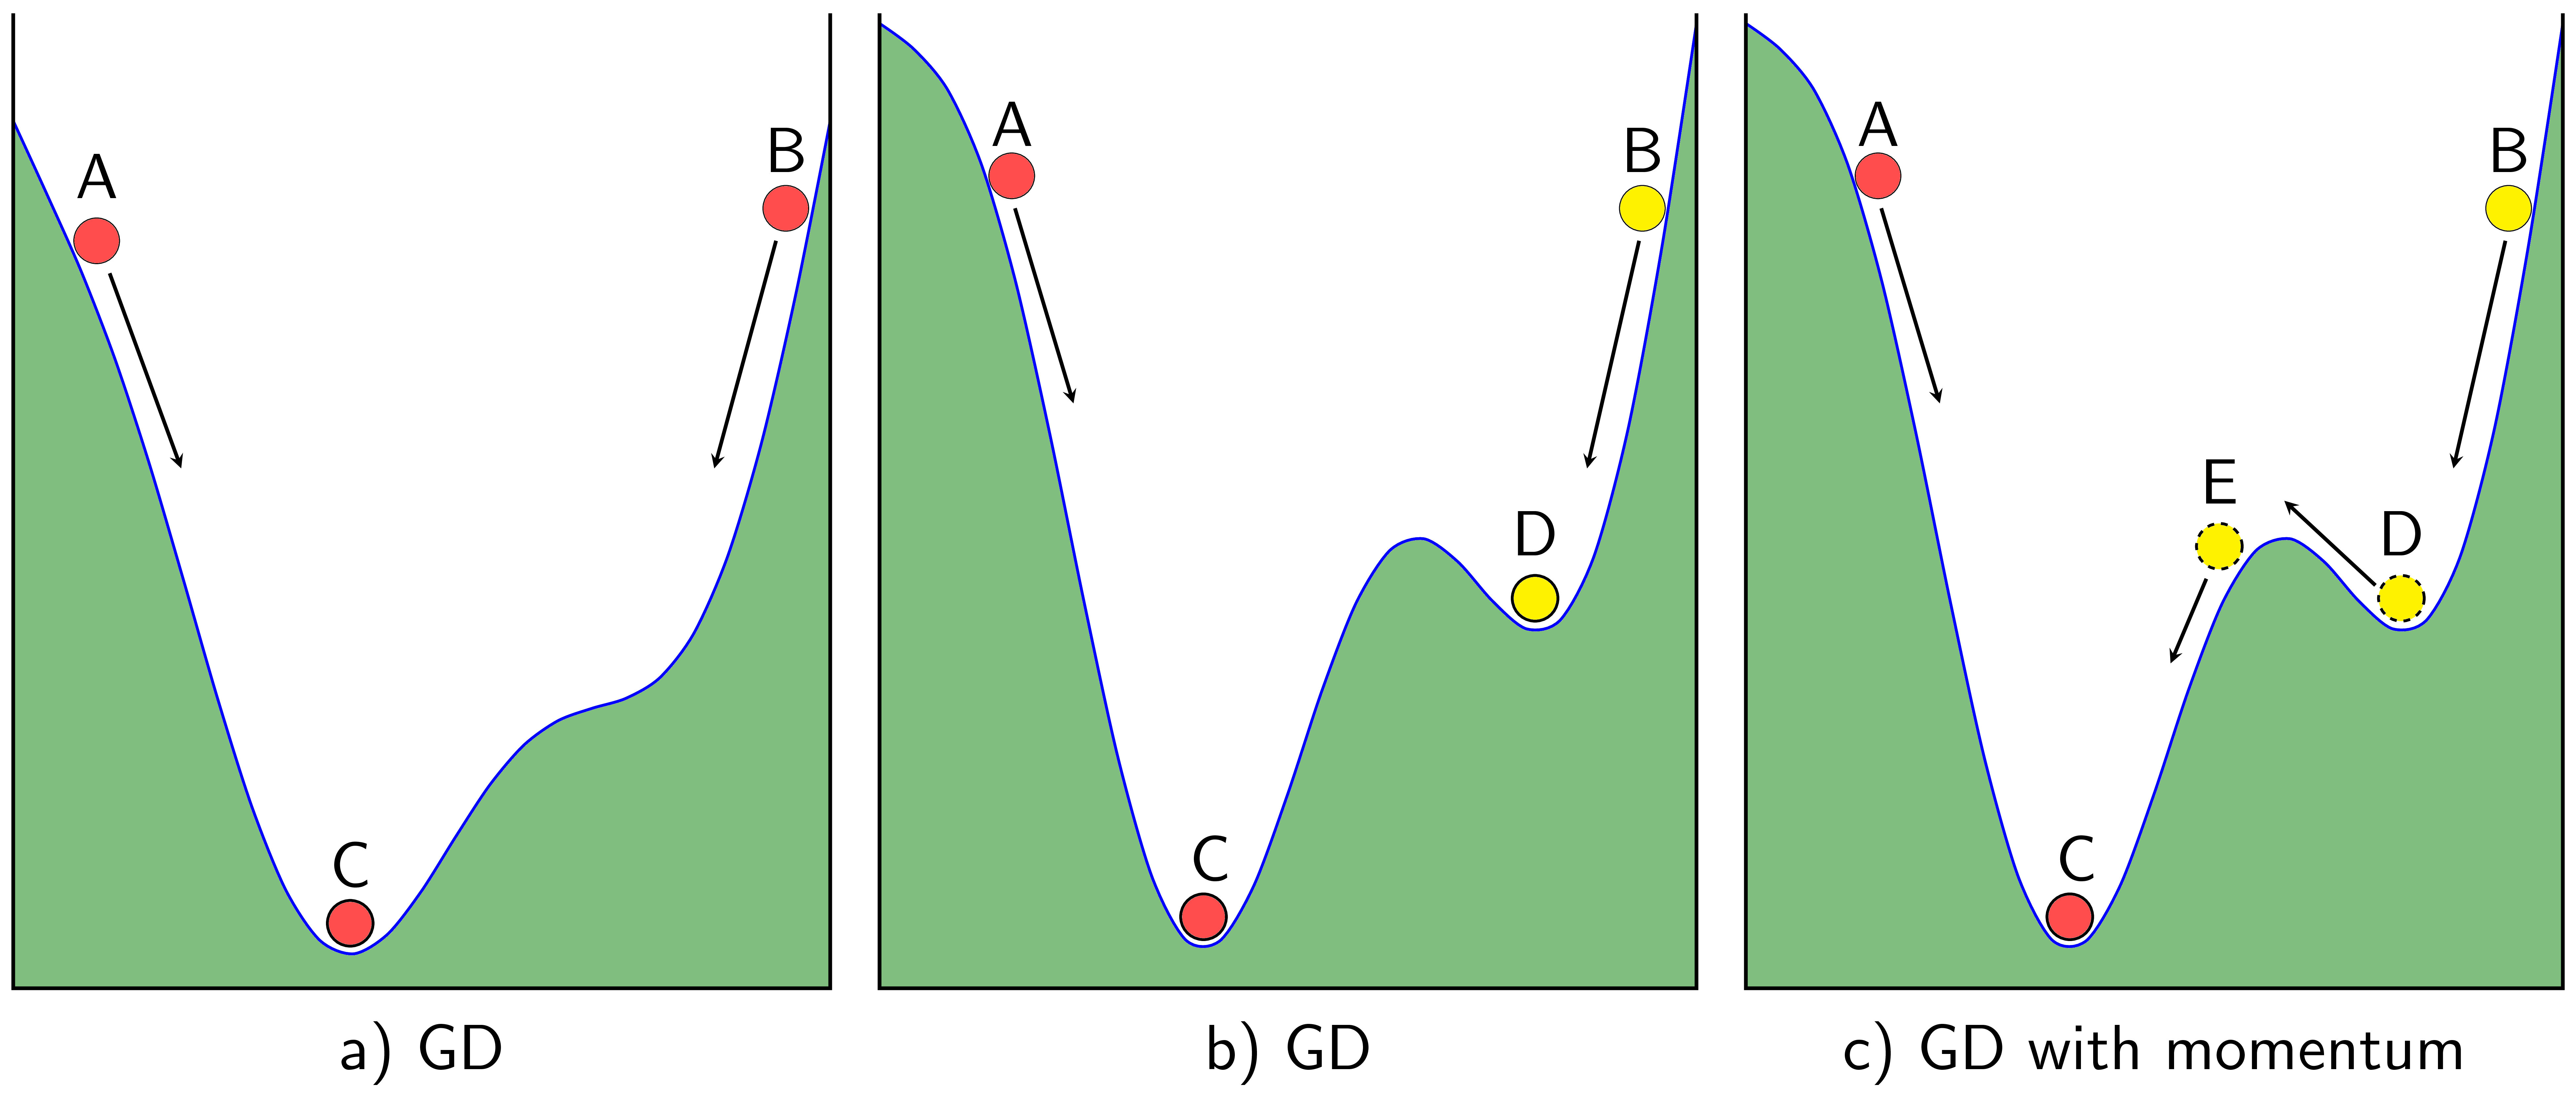
\includegraphics[width = \textwidth]{Chapters/04_Gradientdescent/GD/momentum.png}
    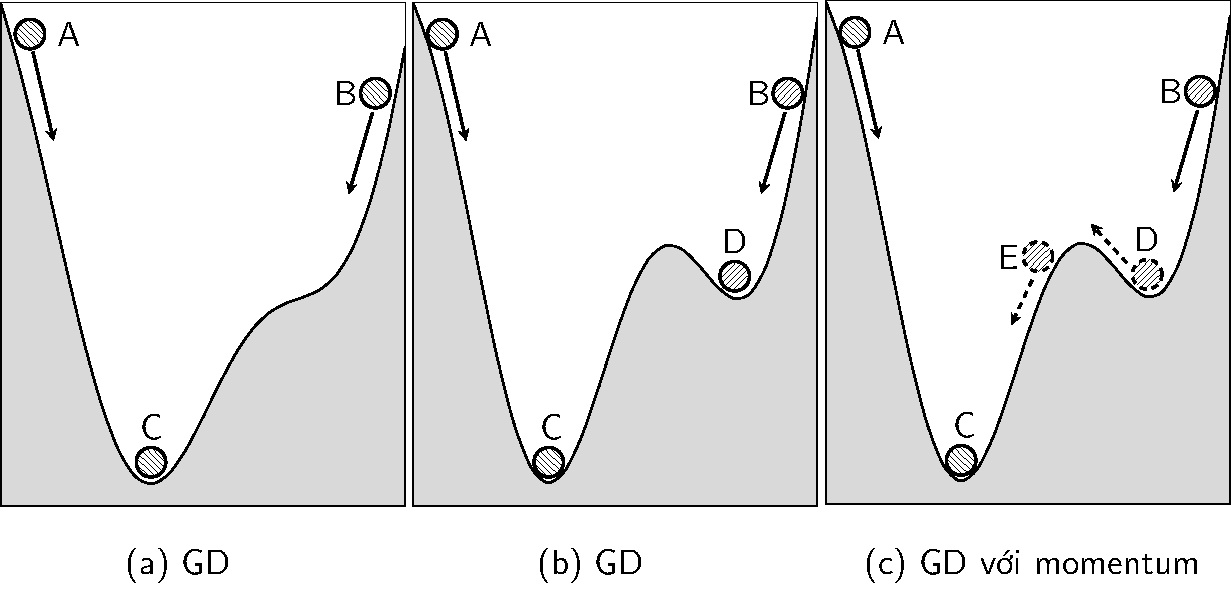
\includegraphics[width = \textwidth]{Chapters/04_GradientDescent/GD/latex/momentum_bw.pdf}
    \caption[]{So sánh GD với các hiện tượng vật lý.}
    \label{fig:8_1}
\end{figure}
Tuy nhiên, nếu bề mặt có hai đáy thung lũng như Hình \ref{fig:8_1}b thì tùy
vào việc đặt bi ở A hoặc B, vị trí cuối cùng tương ứng của bi sẽ ở C hoặc D (giả
sử rằng ma sát đủ lớn và đà không mạnh để bi có thể vượt dốc). Điểm D
là một điểm cực tiểu địa phương, điểm C là điểm cực tiểu toàn cục. 

% \index{momentum}
Vẫn trong Hình \ref{fig:8_1}b, nếu vận tốc ban đầu của bi ở điểm B đủ lớn, nó
vẫn có thể tiến tới dốc bên trái của D do có \textit{đà}. Nếu vận tốc
ban đầu lớn hơn nữa, bi có thể vượt dốc tới điểm E rồi lăn xuống C như trong
Hình~\ref{fig:8_1}c. Dựa trên quan sát này, một thuật toán được ra đời nhằm giúp
GD thoát được các cực tiểu địa phương. Thuật toán đó có tên là \textit{momentum}
(tức \textit{theo đà}).
 
% Đây chính là điều chúng ta mong muốn. Bạn đọc có thể đặt câu hỏi rằng liệu bi lăn từ A tới C có theo \textit{đà} lăn tới E rồi tới D không. Xin trả lời rằng điều này khó xảy ra hơn vì nếu so với dốc DE, dốc CE cao hơn nhiều. 
\index{gradient descent!momentum}
\subsubsection{Gradient descent với momentum}
Làm thế nào để biểu diễn \textit{momentum} dưới dạng toán học?
 
Trong GD, ta cần tính lượng thay đổi ở thời điểm $t$ để cập nhật vị trí
mới cho nghiệm (tức \textit{hòn bi}). Nếu ta coi đại lượng này như vận tốc
$v_t$ trong vật lý, vị trí mới của \textit{hòn bi} sẽ là $\theta_{t+1} =
\theta_{t} - v_t$ với giả sử rằng mỗi vòng lặp là một đơn vị thời gian. Dấu trừ
thể hiện việc phải di chuyển ngược với gradient. Việc tiếp theo là tính đại lượng
$v_t$ sao cho nó vừa mang thông tin của \textit{độ dốc} hiện tại (tức gradient),
vừa mang thông tin của \textit{đà}. Thông tin của đà có thể được hiểu là vận tốc
trước đó $v_{t-1}$ (với giả sử rằng vận tốc ban đầu $v_0=0$). Một cách đơn giản
nhất, ta có thể lấy tổng trọng số của chúng:
\begin{equation} 
\boxed{v_{t}= \gamma v_{t-1} + \eta \nabla_{\theta}J(\theta)} 
\end{equation} 
 Trong đó $\gamma$ là một số dương nhỏ hơn một. Giá trị thường được chọn là khoảng 0.9, $v_{t-1}$ là vận tốc tại thời điểm trước đó, $ \nabla_{\theta}J(\theta)$ chính là độ dốc tại điểm hiện tại. Từ đó, ta có công thức cập nhật nghiệm:
\begin{equation} 
\label{eqn:8_000}
\boxed{\theta \assign \theta - v_t = \theta  - \eta \nabla_{\theta}J(\theta)- \gamma
v_{t-1}}
\end{equation} 
Sự khác nhau giữa GD thông thường và GD với momentem nằm ở thành phần cuối
cùng trong~\eqref{eqn:8_000}. Thuật toán đơn giản này mang lại hiệu quả trong
các bài toán thực tế. % (trong không gian nhiều chiều, cách tính toán cũng hoàn toàn tương tự).

Xét một hàm đơn giản có hai
điểm cực tiểu địa phương, trong đó một điểm là cực tiểu toàn cục:
\begin{equation} 
f(x) = x^2 + 10\sin(x).
\end{equation} 
Hàm số này có đạo hàm là $f'(x) = 2x + 10\cos(x)$. Hình~\ref{fig:8_nomomen} thể
hiện các vị trí trung gian của nghiệm khi không sử dụng momentum. Ta thấy rằng
thuật toán hội tụ nhanh chóng sau chỉ bốn vòng lặp. Tuy nhiên, nghiệm đạt được
không phải là cực tiểu toàn cục. Trong khi đó, Hình~\ref{fig:8_momen} thể hiện các
vị trí trung gian của nghiệm khi có sử dụng momentum. Chúng ta thấy rằng
\textit{hòn bi} vượt được dốc thứ nhất nhờ có \textit{đà}, theo quán tính tiếp
tục vượt qua điểm cực tiểu toàn cục, nhưng trở lại điểm này sau 50 vòng lặp
rồi chuyển động chậm dần quanh đó tới khi dừng hẳn ở vòng lặp thứ 100. Ví dụ này
cho thấy momentum thực sự đã giúp nghiệm thoát được khu vực cực tiểu địa phương.

\begin{figure}[t]
\centering
    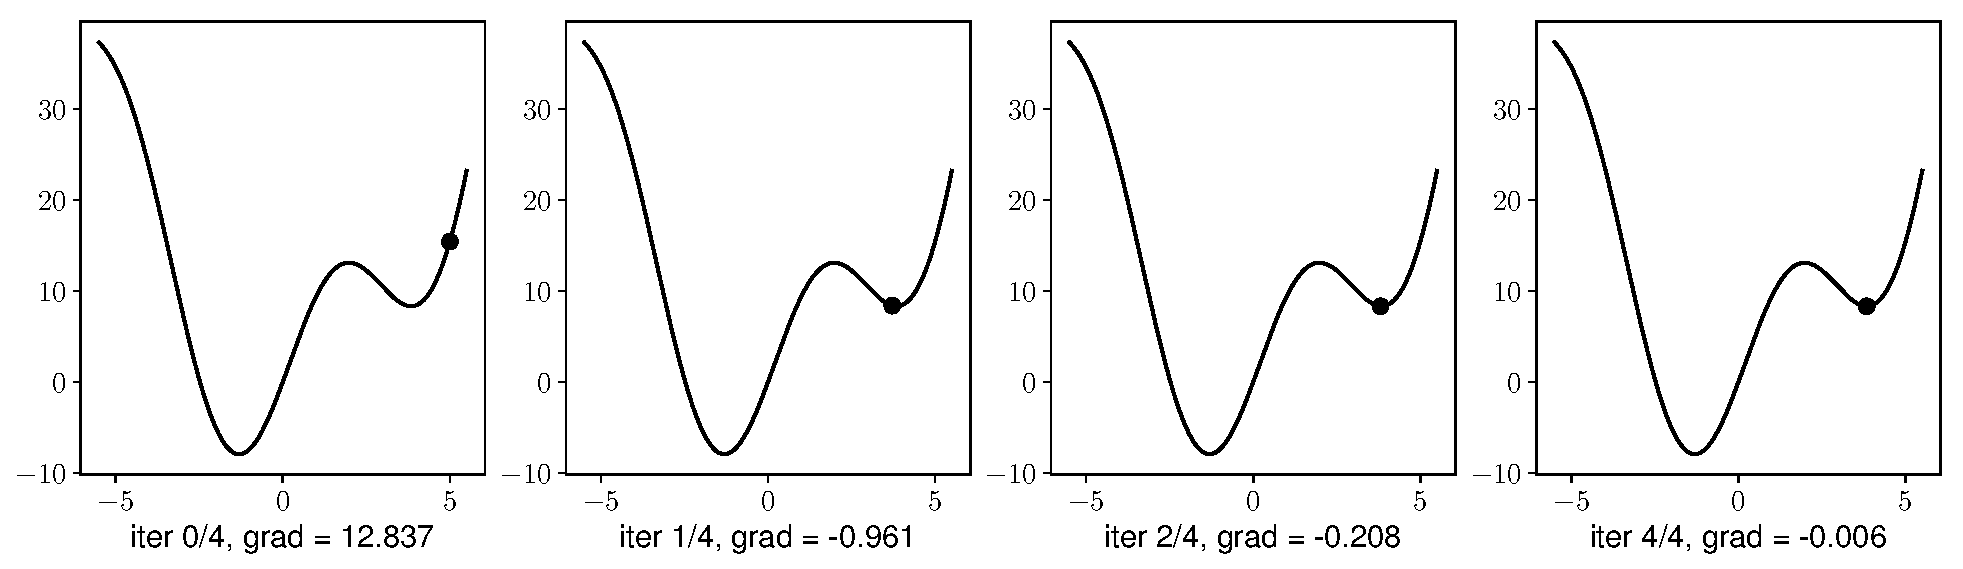
\includegraphics[width = \textwidth]{ebookML_src/src/grad_descent/gd1d_nomomentum.pdf}
    \caption[]{GD thông thường}
    \label{fig:8_nomomen}
\end{figure}

\begin{figure}[t]
\centering
    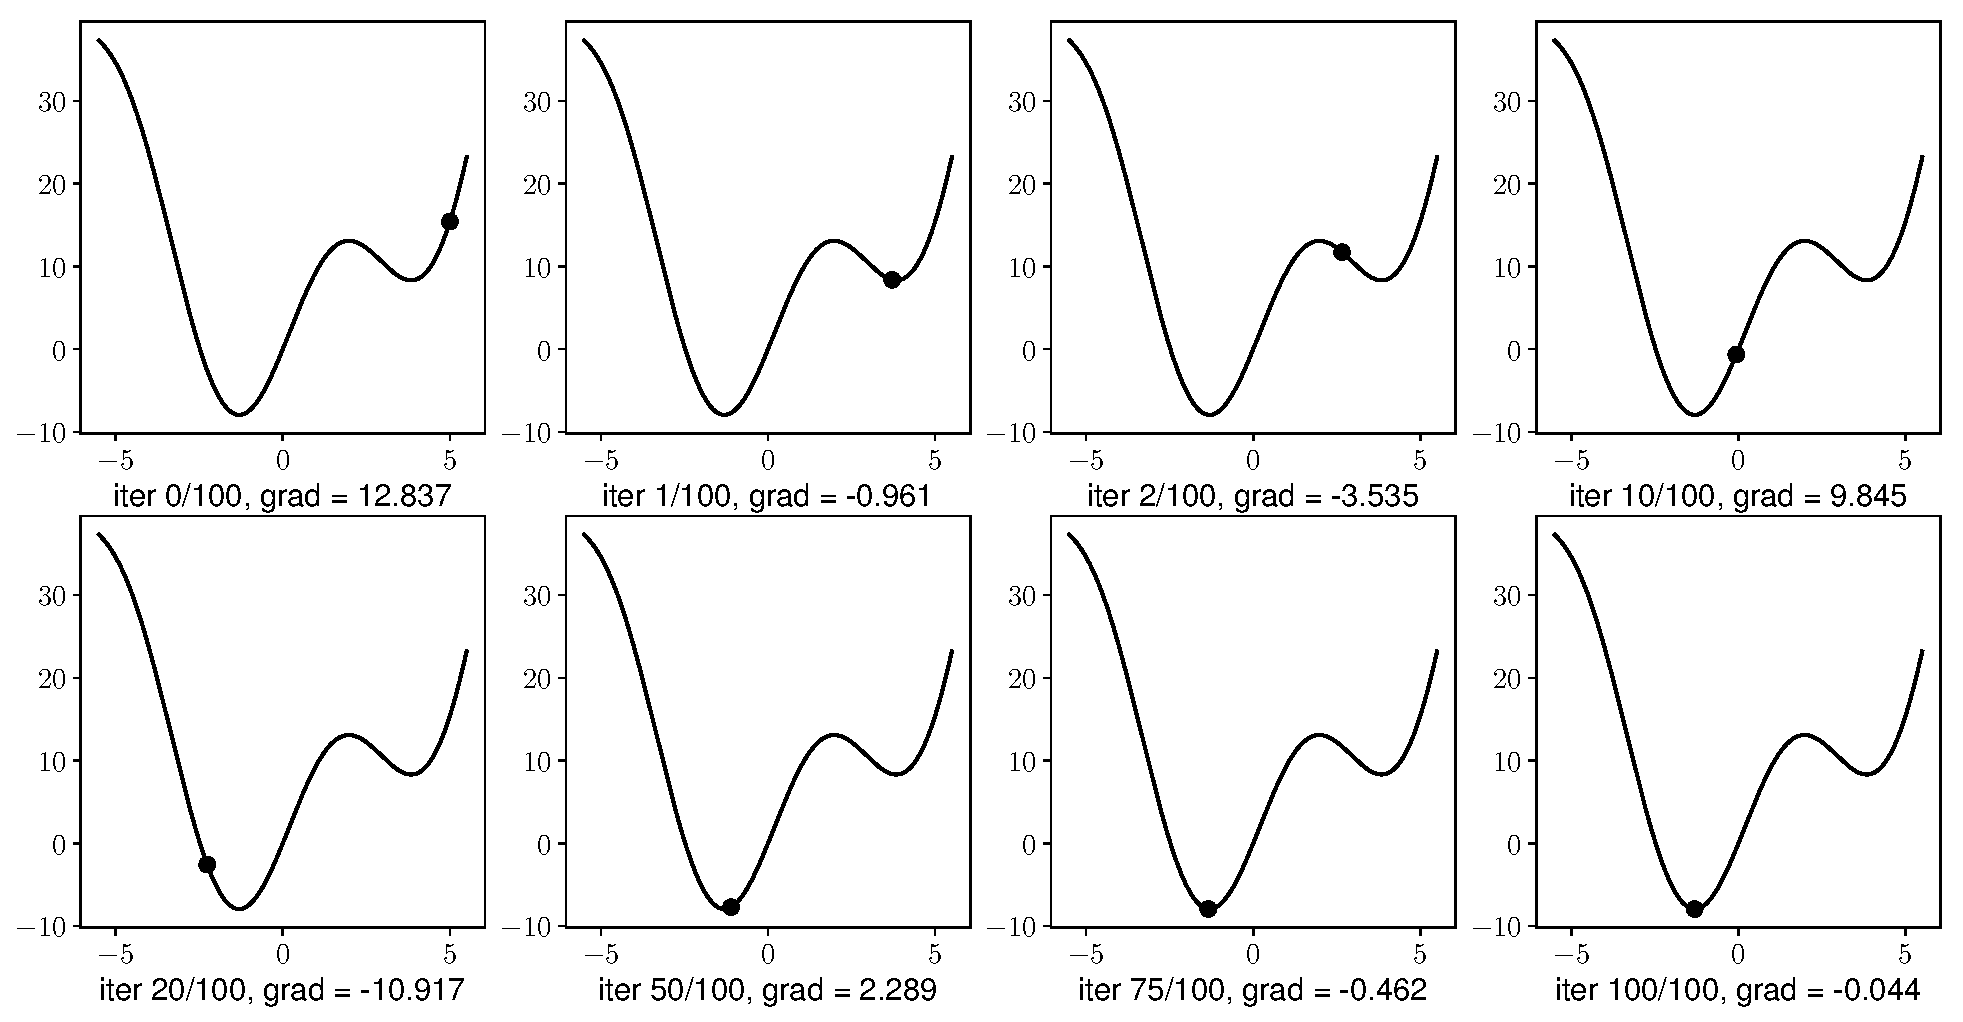
\includegraphics[width = \textwidth]{ebookML_src/src/grad_descent/gd1d_momentum_0.pdf}
    \caption[]{GD với momentum}
    \label{fig:8_momen}
\end{figure}

% <div> 
% <table width = "100%" style = "border: 0px solid white"> 
%    <tr > 
%         <td width="40%" style = "border: 0px solid white">  
%         <img style="display:block;" width = "100%" src = "/assets/GD/nomomentum1d.gif"> 
%          </td> 
%         <td width="40%" style = "border: 0px solid white"> 
%         <img style="display:block;" width = "100%" src = "/assets/GD/momentum1d.gif"> 
%         </td> 
%     </tr> 
% </table>  
% <div class = "thecap"> Hình 2: Minh họa thuật toán GD với Momentum. </div> 
% </div> 
% {\color{red} HÌnh 8.2} 
 
% Hình bên trái là đường đi của nghiệm khi không sử dụng Momentum, thuật toán hội tụ sau chỉ 5 vòng lặp nhưng nghiệm tìm được là nghiệm local minimun. 
 
% Hình bên phải là đường đi của nghiệm khi có sử dụng Momentum, \textit{hòn bi} đã có thể vượt dốc tới khu vực gần điểm global minimun, sau đó dao động xung quanh điểm này, giảm tốc rồi cuối cùng tới đích. Mặc dù mất nhiều vòng lặp hơn, GD với Momentum cho chúng ta nghiệm chính xác hơn. Quan sát đường đi của \textit{hòn bi} trong trường hợp này, chúng ta thấy rằng điều này giống với vật lý hơn! 
 
Nếu biết trước điểm xuất phát \pythoninline{theta}, gradient của hàm mất mát tại
một điểm bất kỳ \pythoninline{grad(theta)}, lượng thông tin lưu trữ từ vận tốc
trước đó \pythoninline{gamma} và tốc độ học \pythoninline{eta}, chúng ta có thể
viết hàm \pythoninline{GD_momentum} như sau:% \newpage 
\newpage 
\begin{lstlisting}[language=Python]
def GD_momentum(grad, theta_init, eta, gamma):
    # Suppose we want to store history of theta
    theta = [theta_init]
    v_old = np.zeros_like(theta_init)
    for it in range(100):
        v_new = gamma*v_old + eta*grad(theta[-1])
        theta_new = theta[-1] - v_new
        if np.linalg.norm(grad(theta_new))/np.array(theta_init).size < 1e-3:
            break
        theta.append(theta_new)
        v_old = v_new
    return theta 
\end{lstlisting}
 
 
\section{Nesterov accelerated gradient}
\index{gradient descent!Nesterov accelerated gradient}
Momentum giúp nghiệm vượt qua được khu vực cực tiểu địa phương. Tuy nhiên, có
một hạn chế có thể thấy trong ví dụ trên. Khi tới gần đích, momemtum khiến
nghiệm dao động một khoảng thời gian nữa trước khi hội tụ. Một kỹ thuật có tên
\textit{Nesterov accelerated gradient} (NAG)~\cite{nesterov2007gradient} giúp
cho thuật toán momentum GD hội tụ nhanh hơn.
 
% \subsection{Ý tưởng chính }
 
Ý tưởng trung tâm của thuật toán là {dự đoán vị trí của nghiệm trước một bước}.
Cụ thể, nếu sử dụng số hạng {momentum} $\gamma v_{t-1}$ để cập nhật thì vị trí
tiếp theo của nghiệm là $\theta - \gamma v_{t-1}$. Vậy, thay vì sử dụng gradient
tại điểm hiện tại, NAG sử dụng gradient tại điểm tiếp theo \textit{nếu sử dụng
momentum}. Ý tưởng này được thể hiện trên Hình~\ref{fig:8_mynag}.
 
% <div class="imgcap"> 
%  <img src ="/assets/GD/nesterov.jpeg" align = "center" width = "800"> 
%  <div class = "thecap"> Ý tưởng của Nesterov accelerated gradient. (Nguồn: <a href="http://cs231n.github.io/neural-networks-3/">CS231n Stanford: Convolutional Neural Networks for Visual Recognition</a>) </div> 
% </div> 
% \begin{figure}[t]
%     % caption on side     
%     \floatbox[{\capbeside\thisfloatsetup{capbesideposition={right,top},capbesidewidth=4cm}}]{figure}[\FBwidth]
%     {\caption{ 
%     Ý tưởng của Nesterov accelerated gradient. (Nguồn: \href{http://cs231n.github.io/neural-networks-3/}{CS231n Stanford: Convolutional Neural Networks for Visual Recognition})
%     }
%     \label{fig:8_nag}}
%     { % figure here
%     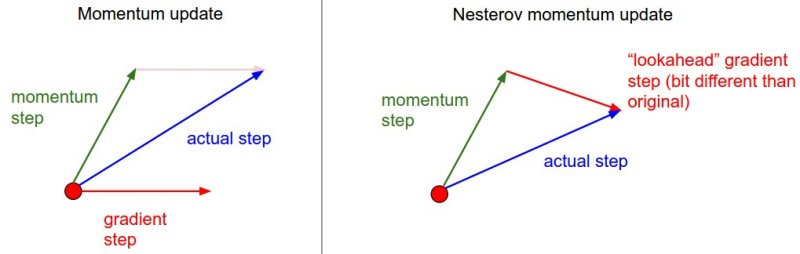
\includegraphics[width=.7\textwidth]{Chapters/04_Gradientdescent/GD/nesterov.jpeg}
%     }
% \end{figure}
%% *****************************************************************************
\begin{figure}[t]
\centering
    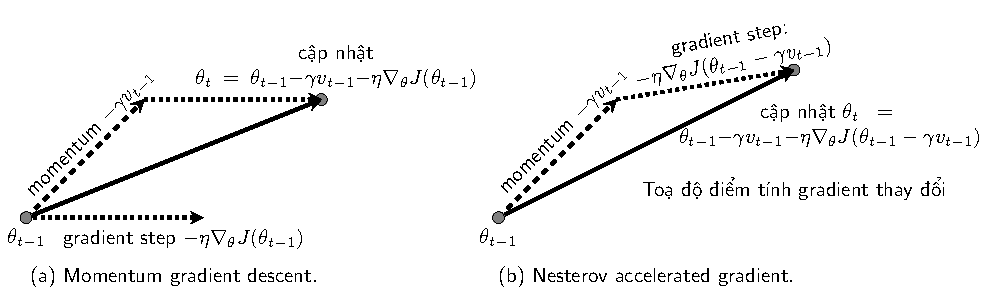
\includegraphics[width = \textwidth]{Chapters/04_GradientDescent/GD/latex/NAG.pdf}
    \caption[]{Ý tưởng của Nesterov accelerated gradient}
    \label{fig:8_mynag}
\end{figure}
%% *****************************************************************************

% \begin{itemize}
% \item Với momentum thông thường, {lượng thay đổi} là tổng của hai vector:
% momentum và gradient ở thời điểm hiện tại. 
 
% \item Với Nesterove momentum, {lượng thay đổi} là tổng của hai vector:
% momentum và gradient tại điểm được dự đoán là vị trí tiếp theo. 

% \end{itemize}
 
% Sự khác nhau giữa momentum và NAG nằm ở điểm lấy đạo hàm. Ở momentum, điểm được
% lấy đạo hàm chính là vị trí hiện tại của nghiệm. Ở NAG, điểm được lấy đạo hàm là
% điểm {tiếp theo nếu sử dụng momentum}.

\subsection{Công thức cập nhật}
 
Công thức cập nhật của NAG được cho như sau:


\myeqnbox{
\begin{eqnarray} 
v_{t} &=& \gamma v_{t-1} + \eta \nabla_{\theta}J(\theta - \gamma v_{t-1}) \\\ 
\theta &\assign& \theta -  v_{t}
\end{eqnarray} 
}

% \begin{tcolorbox}[ams eqnarray]
%     % \begin{eqnarray} 
% v_{t} &=& \gamma v_{t-1} + \eta \nabla_{\theta}J(\theta - \gamma v_{t-1}) \\\ 
% \theta &\assign& \theta -  v_{t}
% \end{eqnarray}
% \end{tcolorbox}


Đoạn code dưới đây thể hiện cách cập nhật nghiệm bằng NAG:
% \newpage
\begin{lstlisting}[language=Python]
def GD_NAG(grad, theta_init, eta, gamma):
    theta = [theta_init]
    v = [np.zeros_like(theta_init)]
    for it in range(100):
        v_new = gamma*v[-1] + eta*grad(theta[-1] - gamma*v[-1])
        theta_new = theta[-1] - v_new
        if np.linalg.norm(grad(theta_new))/np.array(theta_init).size < 1e-3:
            break
        theta.append(theta_new)
        v.append(v_new)
    return theta
\end{lstlisting}

\subsection{Ví dụ minh họa }

\begin{figure}[t]
    \begin{subfigure}{0.49\textwidth}
    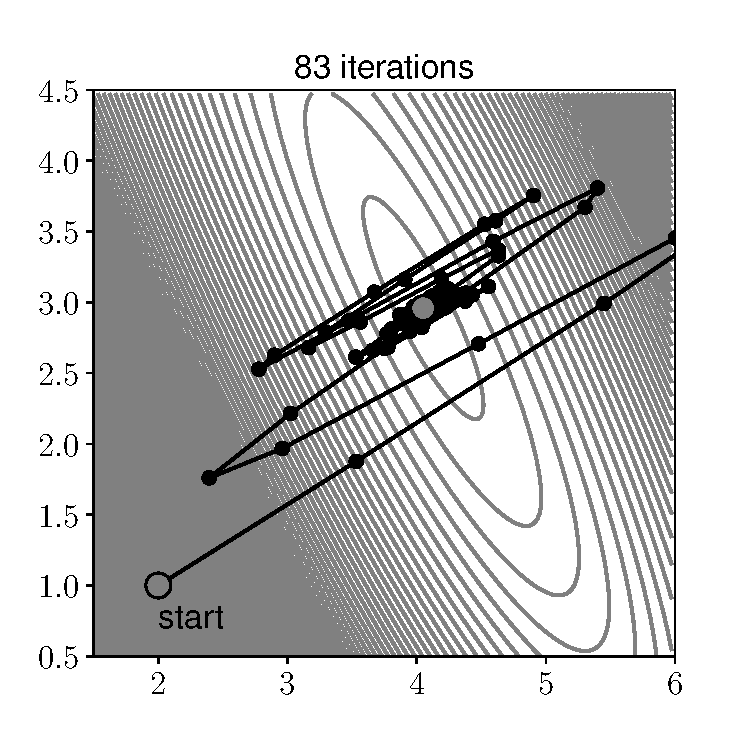
\includegraphics[width=0.99\linewidth]{ebookML_src/src/grad_descent/LR_gd_moment.pdf}
    \caption{GD với momentum.}
    \label{fig:8_momentnaga}
    \end{subfigure}
    \begin{subfigure}{0.49\textwidth}
    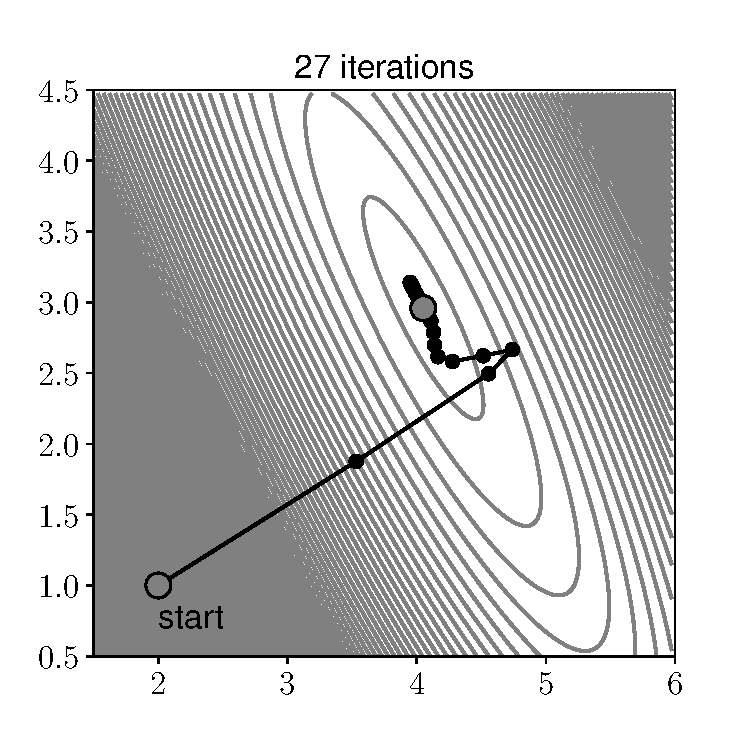
\includegraphics[width=0.99\linewidth]{ebookML_src/src/grad_descent/LR_gd_nag.pdf}
    \caption{GD với NAG.}
    \label{fig:8_momentnagb}
    \end{subfigure}
    \caption{
     Đường đi của nghiệm cho bài toán hồi quy tuyến tính với hai phương pháp
     gradient descent khác nhau. NAG cho nghiệm mượt hơn và nhanh hơn.
    }
    \label{fig:8_momentnag}
\end{figure}

 
Chúng ta cùng áp dụng cả GD với momentum và GD với NAG cho bài toán hồi quy
tuyến tính. Hình~\ref{fig:8_momentnaga} thể hiện đường đi của nghiệm với phương
pháp momentum. Nghiệm đi khá \textit{zigzag} và mất nhiều vòng lặp hơn.
Hình~\ref{fig:8_momentnagb} thể hiện đường đi của nghiệm với phương pháp NAG,
nghiệm hội tụ nhanh hơn và đường đi ít \textit{zigzag} hơn.
 
% (Source code cho \href{https://github.com/ti epvupsu/tiepvupsu.github.io/blob/master/assets/GD/LR%20Momentum.ipynb}{hình bên trái} và \href{https://github.com/tiepvupsu/tiepvupsu.github.io/blob/master/assets/GD/LR%20NAG.ipynb}{ hình bên phải}). 
 
 

 
 
% \section{Biến thể của Gradient descent}
\section{Stochastic gradient descent}
\index{gradient desenct!stochastic gradient descent}
\index{SGD}

% Tôi xin một lần nữa dùng bài toán \href{http://machinelearningcoban.com/2016/12/28/linearregression/}{Linear Regression} làm ví dụ. Hàm mất mát và đạo hàm của nó cho bài toán này lần lượt là (để cho thuận tiện, trong bài này tôi sẽ dùng ký hiệu $\mathbf{X}$ thay cho dữ liệu mở rộng $\bar{\mathbf{X}}$): 
 
% \begin{equation} 
% J(\mathbf{w}) = \frac{1}{2N}\|\mathbf{X}\mathbf{w} - \mathbf{y}\|_2^2 
% \end{equation} 
% \begin{equation} 
% ~~~~ = \frac{1}{2N} \sum_{i=1}^N(\mathbf{x}_i \mathbf{w} - y_i)^2 
% \end{equation} 
% và: 
% \begin{equation} 
% \nabla_{\mathbf{w}} J(\mathbf{w}) = \frac{1}{N}\sum_{i=1}^N \mathbf{x}_i^T(\mathbf{x}_i\mathbf{w} - y_i) 
% \end{equation} 
 
 
\subsection{Batch gradient descent }
\index{batch gradient descent}
Thuật toán GD được đề cập từ đầu chương còn được gọi là \textit{batch gradient
desenct}. Batch ở đây được hiểu là \textit{tất cả}, tức sử dụng {tất cả} các điểm dữ liệu $\mathbf{x}_i$ để cập nhật bộ tham số $\theta$. Hạn chế của
việc này là khi lượng cơ sở dữ liệu lớn, việc tính toán gradient trên toàn bộ dữ
liệu tại mỗi vòng lặp tốn nhiều thời gian.
 
% Cách làm này có một vài hạn chế đối với cơ sở dữ liệu có vô cùng nhiều điểm (hơn 1 tỉ người dùng của facebook chẳng hạn). Việc phải tính toán lại đạo hàm với tất cả các điểm này sau mỗi vòng lặp trở nên cồng kềnh và không hiệu quả. Thêm nữa, thuật toán này được coi là không hiệu quả với \textit{online learning}. 
 
% \index{online learning}
\textit{Online learning} là khi cơ sở dữ liệu được cập nhật liên tục, mỗi lần
tăng thêm vài điểm dữ liệu mới. Việc này yêu cầu mô
hình cũng phải được thay đổi để phù hợp với dữ liệu mới. Nếu thực hiện
batch GD, tức tính lại gradient của hàm mất mát với toàn bộ dữ liệu, độ
phức tạp tính toán sẽ rất cao. Lúc đó, thuật toán có thể không còn mang tính
\textit{online} nữa do mất quá nhiều thời gian tính toán.

Một kỹ thuật đơn giản hơn được sử dụng là \textit{stochastic gradient descent}
(SGD). Thuật toán này có thể gây ra sai số nhưng mang lại lợi ích về mặt tính
toán.

% Trên thực tế, có một thuật toán đơn giản hơn và tỏ ra rất hiệu
% quả, có tên gọi là Stochastic Gradient descent (SGD).

\subsection{Stochastic gradient descent}
\index{vòng lặp -- iteration}
Trong SGD, tại một thời điểm, ta tính gradient của hàm
mất mát dựa trên \textit{chỉ một} điểm dữ liệu $\mathbf{x}_i$ rồi cập nhật
$\theta$. Chú ý rằng hàm mất mát thường được lấy trung bình
trên tất điểm dữ liệu nên gradient tương ứng với một điểm {được kỳ vọng} là khá
gần với gradient tính theo mọi điểm dữ liệu. Sau khi duyệt qua tất cả
các điểm dữ liệu, thuật toán lặp lại quá trình trên. Biến thể đơn giản này trên
thực tế làm việc rất hiệu quả.

% Việc này được thực hiện với từng điểm trên toàn bộ dữ liệu, sau đó
% lặp lại quá trình trên. Thuật toán rất đơn giản này trê thực tế lại làm việc rất
% hiệu quả.

\index{epoch}
\subsubsection{epoch}
\index{học trực tuyến -- online learning}
Mỗi lần duyệt một lượt qua {tất cả} các điểm trên toàn bộ dữ liệu được gọi là
một \textit{epoch}. Với GD thông thường, mỗi epoch ứng với một lần cập nhật
$\theta$. Với SGD, mỗi epoch ứng với $N$ lần cập nhật $\theta$ với $N$ là số
điểm dữ liệu. Một mặt, việc cập nhật $\theta$ theo từng điểm có thể làm giảm tốc
độ thực hiện một epoch. Nhưng mặt khác, với SGD, nghiệm có thể hội tụ sau vài
epoch. Vì vậy, SGD phù hợp với các bài toán có lượng cơ sở dữ liệu lớn và các
bài toán yêu cầu mô hình thay đổi liên tục như \textit{học trực
tuyến}\footnote{\textit{online learning}}. Với một mô hình đã được huấn luyện từ
trước, khi có thêm dữ liệu, ta có thể chạy thêm một vài epoch nữa là đã có
nghiệm hội tụ.

\newnote{}{
Mỗi lần cập nhật nghiệm là một vòng lặp. Mỗi lần duyệt hết toàn bộ dữ
liệu là một \textit{epoch}. Một \textit{epoch} bao gồm nhiều
vòng lặp.
} 
\subsubsection{Thứ tự lựa chọn điểm dữ liệu} 
 
Một điểm cần lưu ý là sau mỗi epoch, thứ tự lấy các dữ liệu cần được xáo trộn để đảm bảo tính ngẫu nhiên.
Việc này cũng ảnh hưởng tới hiệu năng của SGD. Đây cũng chính là lý do thuật
toán này có chứa từ \textit{stochastic}\footnote{\textit{ngẫu nhiên}}.
 
Quy tắc cập nhật của SGD là
\myeqnbox{   
\begin{equation} 
\theta \assign \theta - \eta \nabla_{\theta} J(\theta; \mathbf{x}_i, \by_i)
\end{equation} 
}
Trong đó $J(\theta; \mathbf{x}_i, \by_i) \triangleq J_i(\theta)$ là hàm
mất mát nếu chỉ có một cặp dữ liệu thứ $i$. Các kỹ thuật biến
thể của GD như momentum hay NAG hoàn toàn có thể được áp dụng vào SGD. 


% \subsubsection{Ví dụ với bài toán Linear Regression}
% Với bài toán Linear Regression, $\theta = \mathbf{w}$, hàm mất mát tại một điểm dữ liệu là: 
% \begin{equation} 
% J(\mathbf{w}; \mathbf{x}_i; y_i) = \frac{1}{2}(\mathbf{x}_i \mathbf{w} - y_i)^2 
% \end{equation} 
% Đạo hàm theo $\mathbf{w}$ tương ứng là: 
% \begin{equation} 
% \nabla_{\mathbf{w}}J(\mathbf{w}; \mathbf{x}_i; y_i) = \mathbf{x}_i^T(\mathbf{x}_i \mathbf{w} - y_i) 
% \end{equation} 
% Và dưới đây là hàm số trong python để giải Linear Regression theo SGD: 
 
 
 
 
 
 
% \begin{lstlisting}[language=Python]
% # single point gradient 
% def sgrad(w, i, rd_id): 
%     true_i = rd_id[i] 
%     xi = Xbar[true_i, :] 
%     yi = y[true_i] 
%     a = np.dot(xi, w) - yi 
%     return (xi*a).reshape(2, 1) 
 
% def SGD(w_init, grad, eta): 
%     w = [w_init] 
%     w_last_check = w_init 
%     iter_check_w = 10 
%     N = X.shape[0] 
%     count = 0 
%     for it in range(10): 
%         # shuffle data  
%         rd_id = np.random.permutation(N) 
%         for i in range(N): 
%             count += 1  
%             g = sgrad(w[-1], i, rd_id) 
%             w_new = w[-1] - eta*g 
%             w.append(w_new) 
%             if count%iter_check_w == 0: 
%                 w_this_check = w_new                  
%                 if np.linalg.norm(w_this_check - w_last_check)/len(w_init) < 1e-3:                                     
%                     return w 
%                 w_last_check = w_this_check 
%     return w 
% \end{lstlisting}
 
% Kết quả được cho như hình dưới đây (\href{http://machinelearningcoban.com/2017/01/12/gradientdescent/#quay-lai-voi-bai-toan-linear-regression}{với dữ liệu được tạo giống như ở phần 1}). 
 
% % <div> 
% % <table width = "100%" style = "border: 0px solid white"> 
% %    <tr > 
% %         <td width="40%" style = "border: 0px solid white">  
% %         <img style="display:block;" width = "100%" src = "/assets/GD/LR_SGD_contours.gif"> 
% %          </td> 
% %         <td width="40%" style = "border: 0px solid white"> 
% %         <img style="display:block;" width = "100%" src = "/assets/GD/LR_SGD_loss.png"> 
% %         </td> 
% %     </tr> 
% % </table>  
% % <div class = "thecap"> Trái: đường đi của nghiệm với SGD. Phải: giá trị của loss function tại 50 vòng lặp đầu tiên. </div> 
% % </div> 
% {\color{red} HÌnh 8.4} 
 
% Hình bên trái mô tả đường đi của nghiệm. Chúng ta thấy rằng đường đi khá là \textit{zigzag} chứ không \textit{mượt} như khi sử dụng GD. Điều này là dễ hiểu vì một điểm dữ liệu không thể đại diện cho toàn bộ dữ liệu được. Tuy nhiên, chúng ta cũng thấy rằng thuật toán hội tụ khá nhanh đến vùng lân cận của nghiệm. Với 1000 điểm dữ liệu, SGD chỉ cần gần 3 epoches (2911 tương ứng với 2911 lần cập nhật, mỗi lần lấy 1 điểm). Nếu so với con số 49 vòng lặp (epoches) như kết quả tốt nhất có được bằng GD, thì kết quả này lợi hơn rất nhiều.  
 
% Hình bên phải mô tả hàm mất mát cho toàn bộ dữ liệu sau khi \textit{chỉ} sử dụng 50 điểm dữ liệu đầu tiên. Mặc dù không \textit{mượt}, tốc độ hội tụ vẫn rất nhanh.  
 
% \textit{Thực tế cho thấy chỉ lấy khoảng 10 điểm là ta đã có thể xác định được gần đúng phương trình đường thẳng cần tìm rồi. Đây chính là ưu điểm của SGD - hội tụ rất nhanh.} 
 
 
\subsection{Mini-batch gradient descent}
\index{gradient descent!mini-batch}
\index{gradient descent!kích thước batch -- batch size}
Khác với SGD, mini-batch GD sử dụng $1 < k < N$ điểm dữ liệu để cập nhật ở mỗi
vòng lặp. Giống với SGD, mini-batch GD bắt đầu mỗi epoch bằng việc xáo trộn ngẫu
nhiên dữ liệu rồi chia toàn bộ dữ liệu thành các {mini-batch}, mỗi {mini-batch}
có $k$ điểm dữ liệu (trừ mini-batch cuối có thể có ít hơn nếu $N$ không chia hết
cho $k$). Ở mỗi vòng lặp, một mini-batch được lấy ra để tính toán gradient rồi
cập nhật $\theta$. Khi thuật toán chạy hết dữ liệu một lượt cũng là khi kết thúc
một epoch. Như vậy, {một epoch} bao gồm xấp xỉ $N/k$ vòng lặp. Giá trị $k$ được
gọi là \textit{kích thước batch} (không phải \textit{kích thước mini-batch}) được chọn trong khoảng khoảng từ vài chục đến vài trăm.
 
Hình~\ref{fig:7_minibatch} là ví dụ về giá trị của hàm mất mát của một mô hình
phức tạp hơn khi sử dụng mini-batch GD. Mặc dù giá trị của hàm mất mát sau các
vòng lặp không luôn luôn giảm, nhìn chung giá trị này có xu hướng giảm và hội
tụ.

% ******************************************************************************
\begin{figure}[t]
    % caption on side     
   
    \floatbox[{\capbeside\thisfloatsetup{capbesideposition={right,top},capbesidewidth=5cm}}]{figure}[\FBwidth]
    {\caption{ 
    Ví dụ về giá trị hàm mất mát sau mỗi vòng lặp khi sử dụng mini-batch
    gradient descent.
    Hàm mất mát dao động sau mỗi lần cập
    nhật nhưng nhìn chung giảm dần và có xu hướng hội tụ.
    }
    \label{fig:7_minibatch}}
    { % figure here
    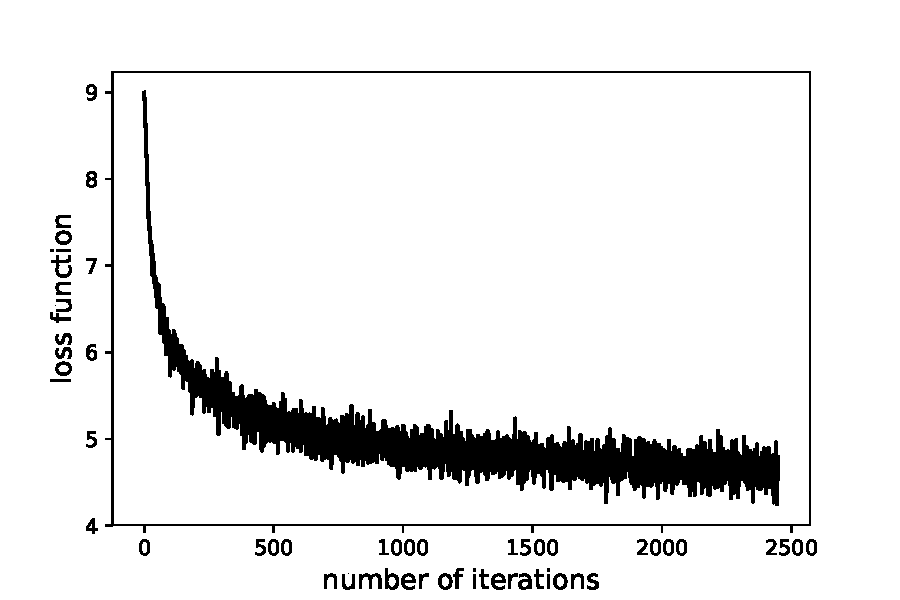
\includegraphics[width=.65\textwidth]{ebookML_src/src/multiclasssvm/loss_history.pdf}
    }
\end{figure}
% ******************************************************************************
 
% <div class="imgcap"> 
%  <img src ="https://upload.wikimedia.org/wikipedia/commons/f/f3/Stogra.png" align = "center" width = "400"> 
%  <div class = "thecap"> Hàm mất mát \textit{nhảy lên nhảy xuống} (fluctuate) sau mỗi lần cập nhật nhưng nhìn chung giảm dần và có xu hướng hội tụ về cuối. (Nguồn: <a href = "https://en.wikipedia.org/wiki/Stochastic_gradient_descent">Wikipedia</a>). </div> 
% </div> 
% {\color{red} HÌnh 8.5} 
 
% Để có thêm thông tin chi tiết hơn, bạn đọc có thể tìm trong \href{http://sebastianruder.com/optimizing-gradient-descent/index.html#stochasticgradientdescent}{bài viết rất tốt này}.  
 
 

% \subsection{Các thuật toán khác}



% Ngoài hai thuật toán trên, có rất nhiều thuật toán nâng cao khác được sử dụng trong các bài toán thực tế, đặc biệt là các bài toán Deep Learning. Có thể nêu một vài từ khóa như Adagrad, Adam, RMSprop,... Tôi sẽ không đề cập đến các thuật toán đó trong bài này mà sẽ dành thời gian nói tới nếu có dịp trong tương lai, khi blog đã đủ lớn và đã trang bị cho các bạn một lượng kiến thức nhất định.  
 

 
\section{Thảo luận}
\subsection{Điều kiện dừng thuật toán}
\index{gradient descent!điều kiện dừng --stopping criteria}
Khi nào thì nên dừng thuật toán GD? 
 
Trong thực nghiệm, chúng ta có thể kết hợp các phương pháp sau:
\begin{enumerate}
    \item  Giới hạn số vòng lặp. Nhược điểm của cách
    làm này là thuật toán có thể dừng lại trước khi nghiệm đủ tốt. Tuy nhiên,
    đây là phương pháp phổ biến nhất và cũng đảm bảo được chương trình chạy
    không quá lâu.

    \item  So sánh gradient của hàm mất mát tại hai lần cập nhật liên tiếp, khi nào
    giá trị này đủ nhỏ thì dừng lại.

    \item  So sánh giá trị của hàm mất mát sau một vài epoch, khi nào sự sai
    khác đủ nhỏ thì dừng lại. Nhược điểm của phương pháp này là nếu hàm mất mát có
    dạng {bằng phẳng} tại một điểm không phải cực tiểu địa phương, thuật
    toán sẽ dừng lại trước khi đạt giá trị mong muốn.

    \item Vừa chạy GD, vừa kiểm tra kết quả. Một kỹ thuật khác thường
    được sử dụng là cho thuật toán chạy với số lượng vòng lặp lớn. Trong quá
    trình chạy, chương trình thường xuyên kiểm tra chất lượng mô hình trên tập
    huấn luyện và tập xác thực. Đồng thời, mô hình sau một vài vòng lặp được lưu
    lại trong bộ nhớ. Nếu ta thấy chất lượng mô hình bắt đầu giảm trên tập xác thực thì dừng lại. Đây chính là kỹ thuật \textit{early stoping} đã đề cập trong Chương~\ref{cha:overfitting}.

    % \item Để hạn chế lượng tính toán, viê

    % \item  Trong SGD và mini-batch GD, cách thường dùng là so sánh nghiệm sau
    % một vài lần cập nhật. 
    % Trong đoạn code Python phía trên về SGD, tôi áp dụng
    % việc so sánh này mỗi khi nghiệm được cập nhật 10 lần. Việc làm này cũng tỏ
    % ra khá hiệu quả.
\end{enumerate}
 
 
 
 
% \section{Một phương pháp tối ưu đơn giản khác: Newton's method}
 
% Nhân tiện đang nói về tối ưu, tôi xin giới thiệu một phương pháp nữa có cách giải thích đơn giản: Newton's method. Các phương pháp GD tôi đã trình bày còn được gọi là first-order methods, vì lời giải tìm được dựa trên đạo hàm bậc nhất của hàm số. Newton's method là một second-order method, tức lời giải yêu cầu tính đến đạo hàm bậc hai. 
 
 
% Nhắc lại rằng, cho tới thời điểm này, chúng ta luôn giải phương trình đạo hàm của hàm mất mát bằng 0 để tìm các điểm local minimun. (Và trong nhiều trường hợp, coi nghiệm tìm được là nghiệm của bài toán tìm giá trị nhỏ nhất của hàm mất mát). Có một thuật toán nối tiếng giúp giải bài toán $f(x) = 0$, thuật toán đó có tên là Newton's method. 
 
 
 
% \subsection{Newton's method cho giải phương trình $f(x) = 0$}
 
% Thuật toán Newton's method được mô tả trong hình động minh họa dưới đây: 
 
% <div class="imgcap"> 
%  <img src ="https://upload.wikimedia.org/wikipedia/commons/e/e0/NewtonIteration_Ani.gif" align = "center" width = "500"> 
%  <div class = "thecap"> Hình 3: Minh họa thuật toán Newton's method trong giải phương trình. (  Nguồn: <a href = "https://en.wikipedia.org/wiki/Newton's_method"> Newton's method - Wikipedia</a>).</div> 
% </div> 
 
 
% Ý tưởng giải bài toán $f(x) = 0$ bằng phương pháp Newton's method như sau. Xuất phát từ một điểm $x_0$ được cho là gần với nghiệm $x^\*$. Sau đó vẽ đường tiếp tuyến (mặt tiếp tuyến trong không gian nhiều chiều) với đồ thị hàm số $y = f(x)$ tại điểm trên đồ thị có hoành độ $x_0$. Giao điểm $x_1$ của đường tiếp tuyến này với trục hoành được xem là gần với nghiệm $x^\*$ hơn. Thuật toán lặp lại với điểm mới $x_1$ và cứ như vậy đến khi ta được $f(x_t) \approx 0$. 
 
 
% Đó là ý nghĩa hình học của Newton's method, chúng ta cần một công thức để có thể dựa vào đó để lập trình. Việc này không quá phức tạp với các bạn thi đại học môn toán ở VN. Thật vậy, phương trình tiếp tuyến với đồ thị của hàm $f(x)$ tại điểm có hoành độ $x_t$ là: 
% \begin{equation} 
% y = f'(x_t)(x - x_t) + f(x_t) 
% \end{equation} 
% Giao điểm của đường thẳng này với trục $x$ tìm được bằng cách giải phương trình vế phải của biểu thức trên bằng 0, tức là: 
% \begin{equation} 
% x = x_t - \frac{f(x_t)}{f'(x_t)} \triangleq x_{t+1} 
% \end{equation} 
 
 
% \subsection{Newton's method trong bài toán tìm local minimun}
% Áp dụng phương pháp này cho việc giải phương trình $f'(x) = 0$ ta có: 
% \begin{equation} 
% x_{t+1} = x_t -(f"(x_t))^{-1}{f'(x_t)} 
% \end{equation} 
 
% Và trong không gian nhiều chiều với $\theta$ là biến: 
% \begin{equation} 
% \theta = \theta - \mathbf{H}(J(\theta))^{-1} \nabla_{\theta} J(\theta) 
% \end{equation} 
% trong đó $\mathbf{H}(J(\theta))$ là đạo hàm bậc hai của hàm mất mất (còn gọi là \href{https://en.wikipedia.org/wiki/Hessian_matrix}{Hessian matrix}). Biểu thức này là một ma trận nếu $\theta$ là một vector. Và $\mathbf{H}(J(\theta))^{-1}$ chính là nghịch đảo của ma trận đó.  
 
 
 
% \subsection{Hạn chế của Newton's method}
% \item Điểm xuất phát phải \textit{rất} gần với nghiệm $x^\*$. 
% Ý tưởng sâu xa hơn của Newton's method là dựa trên khai triển Taylor của hàm số $f(x)$ tới đạo hàm thứ nhất: 
% \begin{equation} 
% 0 = f(x^\}) \approx f(x_t) + f'(x_t)(x_t - x^\}) 
% \end{equation} 
% Từ đó suy ra: $x^\} \approx x_t - \frac{f(x_t)}{f'(x_t)}$.  
% Một điểm rất quan trọng, khai triển Taylor chỉ đúng nếu $x_t$ rất gần với $x^\*$! 
% Dưới đây là một ví dụ kinh điển trên Wikipedia về việc Newton's method cho một dãy số phân kỳ (divergence). 
% <div class="imgcap"> 
%  <img src ="https://upload.wikimedia.org/wikipedia/commons/thumb/f/f1/NewtonsMethodConvergenceFailure.svg/300px-NewtonsMethodConvergenceFailure.svg.png" align = "center" width = "400"> 
%  <div class = "thecap"> Hình 4: Nghiệm là một điểm gần -2. Tiếp tuyến của đồ thị hàm số tại điểm có hoành độ bằng 0 cắt trục hoành tại 1, và ngược lại. Trong trường hợp này, Newton's method không bao giờ hội tụ. (Nguồn: <a href = "https://en.wikipedia.org/wiki/Newton's_method">Wikipedia</a>). </div> 
% </div> 
 
% \item Nhận thấy rằng trong việc giải phương trình $f(x) = 0$, chúng ta có đạo hàm ở mẫu số. Khi đạo hàm này gần với 0, ta sẽ được một đường thằng song song hoặc gần song song với trục hoành. Ta sẽ hoặc không tìm được giao điểm, hoặc được một giao điểm ở vô cùng. Đặc biệt, khi nghiệm chính là điểm có đạo hàm bằng 0, thuật toán gần như sẽ không tìm được nghiệm! 
 
% \item Khi áp dụng Newton's method cho bài toán tối ưu trong không gian nhiều chiều, chúng ta cần tính nghịch đảo của Hessian matrix. Khi số chiều và số điểm dữ liệu lớn, đạo hàm bậc hai của hàm mất mát sẽ là một ma trận rất lớn, ảnh hưởng tới cả memory và tốc độ tính toán của hệ thống. 
 
 
 
% \section{Kết luận}
% Qua hai bài viết về Gradient descent này, tôi hy vọng các bạn đã hiểu và làm quen với một thuật toán tối ưu được sử dụng nhiều nhất trong Machine Learning và đặc biệt là Deep Learning. Còn nhiều biến thể khác khá thú vị về GD (mà rất có thể tôi chưa biết tới), nhưng tôi xin phép được dừng chuỗi bài về GD tại đây và tiếp tục chuyển sang các thuật toán thú vị khác.  
 
% Hy vọng bài viết có ích với các bạn. 
 
 
\subsection{Đọc thêm}

Mã nguồn trong chương này có thể được tìm thấy tại
\url{https://goo.gl/RJrRv7}. 

Ngoài các thuật toán đã đề cập trong chương này, có nhiều thuật toán khác giúp
cải thiện GD được đề xuất gần đây~\cite{ruder2016overview}. Bạn
đọc có thể tham khảo thêm AdaGrad~\cite{duchi2011adaptive},
RMSProp~\cite{tieleman2012lecture}, Adam~\cite{kingma2014adam},...

Các trang web và video dưới đây cũng là các tài liệu tốt về GD.
\begin{enumerate}
    % \item \href{https://en.wikipedia.org/wiki/Newton's_method}{Newton's method - Wikipedia} 
 
    \item \textit{An overview of gradient descent optimization algorithms}
    (\url{https://goo.gl/AGwbbg}).
 
    \item \textit{Stochastic Gradient descent -- Wikipedia}
    (\url{https://goo.gl/pmuLzk}). 

    \item \textit{Stochastic gradient descent -- Andrew Ng} (\url{https://goo.gl/jgBf2N}). 
     
    \item  \textit{An Interactive Tutorial on Numerical Optimization}
    (\url{https://goo.gl/t85mvA}). 

    \item \textit{Machine Learning cơ bản, Bài 7, 8} (\url{https://goo.gl/US17PP}).

\end{enumerate}
